\documentclass[12pt]{article}
\usepackage{setspace}
\usepackage{titlesec}
\usepackage{graphicx}
\usepackage{amsmath}
\usepackage{amssymb}
\usepackage{hyperref}
\usepackage{booktabs}
\usepackage{listings}
\usepackage{xcolor}
\usepackage{enumitem}
\usepackage{array}
\usepackage{caption}
\usepackage{geometry}
\usepackage{multirow}
\geometry{margin=1in}

\lstset{
  basicstyle=\ttfamily\small,
  backgroundcolor=\color{gray!10},
  frame=single,
  breaklines=true,
  columns=fullflexible,
  keepspaces=true
}

\hypersetup{
    colorlinks=true,
    linkcolor=blue,
    urlcolor=blue,
    citecolor=blue
}

\begin{document}

% ─────────────────────────────────────────────
%  TITLE PAGE
% ─────────────────────────────────────────────
\begin{center}
    
\includegraphics[width=9cm,height=2cm]{Picture1.png}
\end{center}
\vspace{0.5cm}
\begin{center}
    \textbf{\Large School of Engineering, Applied Sciences, and Technology} \\[0.5cm]
    \textbf{\large MAI 604 -- Deep Learning} \\[0.3cm]
    \textbf{\large Course Project}
\end{center}
\vspace{1cm}
\noindent
\begin{tabular}{ll}
\textbf{Course Code:} MAI 604 & \textbf{Course Name:} Deep Learning \\
\textbf{Date:} 04/18/26       & \textbf{Time:} TBD \\
\textbf{Location:} TBD        & \textbf{Instructor(s):} Dr. Firuz Kamalov \\
\textbf{Number of Students:} 3 & \textbf{Number of Pages:} TBD \\
\end{tabular}
\vspace{1cm}
\begin{center}
\textbf{\large Project Title}
\end{center}
\vspace{0.5cm}
\begin{center}
\textbf{\Large Predicting Bitcoin Honestly: Log-Return Targets, Walk-Forward Validation, and Why Sub-1 Percentage MAPE Isn't What It Seems}
\end{center}
\vspace{1cm}
\begin{flushleft}
\textbf{Students Names:} \\[0.2cm]
\text{Shamsa Alsuwaidi} \\[0.1cm]
\text{Saeeda Amer} \\[0.1cm]
\text{Amna Aljaroodi} \\[0.2cm]
\textbf{University IDs:} \\[0.2cm]
\text{20250007177} \\[0.1cm]
\text{20250006821} \\[0.1cm]
\text{20250007933} \\[0.2cm]
\end{flushleft}

\newpage

% ─────────────────────────────────────────────
%  TABLE OF CONTENTS
% ─────────────────────────────────────────────
\tableofcontents
\newpage

% ─────────────────────────────────────────────
\section{Background to Study}
% ─────────────────────────────────────────────

\subsection{Overview of Bitcoin and Cryptocurrency Markets}

Bitcoin (BTC) is a decentralized digital currency introduced in 2008 by an anonymous entity known as Satoshi Nakamoto \cite{nakamoto2008}. Operating on a peer-to-peer network secured by blockchain technology, Bitcoin allows trustless financial transactions without reliance on any central authority such as a bank or government. Since its inception, Bitcoin has grown from an experimental technology to one of the world's most widely traded financial assets, with a market capitalization that has at various points exceeded one trillion US dollars. Following the approval of spot Bitcoin exchange-traded products by the United States Securities and Exchange Commission in January 2024, Bitcoin reached historical highs above \$94{,}000, reflecting its transition from a speculative retail asset to an institutionally recognized one \cite{wu2025cfa}.

The cryptocurrency market is distinguished by several characteristics that set it apart from traditional financial markets. Unlike stock exchanges, cryptocurrency markets operate continuously, 24 hours a day, 7 days a week, across the globe. This perpetual operation, combined with relatively limited market depth compared to traditional assets and the absence of circuit breakers, contributes to the extreme price volatility that characterizes Bitcoin's trading history. The asset has experienced multiple full price cycles, including a rise to approximately \$20{,}000 in late 2017, a subsequent crash below \$4{,}000 in 2018, a dramatic surge past \$60{,}000 in 2021, a 2022 crash tied to the collapse of several exchanges, and a renewed rally through 2024--2025. This regime diversity makes Bitcoin a particularly challenging forecasting target --- any single static evaluation window can easily over- or under-state model capability depending on which regime it happens to land in.

\subsection{Problem Statement}

Accurate prediction of Bitcoin prices has significant financial and academic value. For individual investors and institutional traders, even marginal improvements in predictive accuracy can translate to substantial financial returns. From a scientific perspective, Bitcoin represents a challenging testbed for forecasting methods due to its non-stationary dynamics, heavy-tailed return distribution, and susceptibility to exogenous shocks such as regulatory announcements and macroeconomic events.

Traditional financial forecasting methods, including ARIMA (AutoRegressive Integrated Moving Average) and GARCH (Generalized Autoregressive Conditional Heteroskedasticity) models, rely on assumptions of linearity and stationarity that are routinely violated by cryptocurrency price series \cite{jin2025tcn}. Deep learning models, capable of learning highly non-linear mappings from high-dimensional input spaces, have emerged as compelling alternatives. However, na\"{i}vely applying deep networks to raw price data is prone to two silent failure modes that this project explicitly addresses: (i) \textit{data leakage} via scalers fitted on the combined train-test data, and (ii) \textit{non-stationarity} arising when a model trained on prices in one regime must extrapolate into a regime with fundamentally different price levels. Both issues are discussed in detail in Section~\ref{sec:methodology}.

\subsection{Motivation}

This project is motivated by four observations:
\begin{enumerate}[leftmargin=*]
    \item The inherent complexity and regime-dependence of Bitcoin dynamics render classical statistical models insufficient for reliable prediction.
    \item Recent advances in deep learning architectures --- attention-based recurrent networks, hybrid convolutional-transformer models, and temporal convolutional networks --- have demonstrated state-of-the-art performance on sequential financial data.
    \item Many published Bitcoin-prediction results reporting very low MAPE values rely on evaluation protocols that contain subtle forms of information leakage. A controlled, leak-free study is valuable for establishing realistic performance expectations.
    \item A broad feature set drawn from on-chain indicators, cross-asset prices, macroeconomic variables and market-sentiment signals has been shown to enhance predictive power beyond what price history alone provides \cite{wu2025cfa,jin2025tcn}.
\end{enumerate}

\subsection{Scope of the Project}

This project predicts the \emph{next three days'} Bitcoin closing prices (Day+1, Day+2, Day+3) using approximately nine years of historical BTC-USD data from January 2017 through April 2026. Four deep learning architectures are implemented, trained under identical conditions, and compared head-to-head: a Deep Neural Network (DNN) with a feature-attention gate; an LSTM with temporal self-attention; a hybrid CNN-Transformer; and a Temporal Convolutional Network (TCN). Two ensemble strategies are also evaluated. Evaluation includes static chronological split metrics, walk-forward validation across twenty re-training windows spanning 2019--2025, feature-group ablation, Diebold--Mariano tests for statistical significance, and Monte Carlo Dropout uncertainty quantification.

% ─────────────────────────────────────────────
\section{Literature Review}
% ─────────────────────────────────────────────

\subsection{Traditional Approaches to Financial Forecasting}

Time-series forecasting in finance has a long history rooted in econometric models. Box and Jenkins' ARIMA framework \cite{box2015} provided the dominant paradigm for several decades, modelling a time series as a function of its own lagged values and lagged forecast errors. While effective for stationary linear processes, ARIMA models have been consistently shown to struggle with the highly volatile, non-linear dynamics of cryptocurrency prices. GARCH-family models extended this framework to capture time-varying volatility, but their assumptions regarding the distributional form of innovations remain problematic for assets like Bitcoin, which exhibits heavy tails and skewness in its return distribution. Katsiampa \cite{katsiampa2017} evaluated various GARCH specifications for Bitcoin volatility but found that accurate point-price prediction remained elusive.

\subsection{Machine Learning in Cryptocurrency Prediction}

The introduction of classical machine-learning techniques opened new avenues for financial forecasting. Support Vector Regression (SVR), Random Forests, and Gradient Boosting methods were applied to Bitcoin prediction tasks with moderate success \cite{madan2015,chen2020}. Chen, Li and Sun \cite{chen2020} specifically demonstrated that sample-dimension engineering --- the careful construction of input features --- often matters more than the choice of classical model family.

\subsection{Deep Learning for Sequential Financial Data}

\subsubsection{Recurrent Neural Networks and LSTM}

The introduction of Long Short-Term Memory (LSTM) networks by Hochreiter and Schmidhuber \cite{hochreiter1997} addressed the vanishing gradient problem that plagued standard recurrent networks, enabling effective learning of long-range temporal dependencies. Fischer and Krauss \cite{fischer2018} applied deep LSTMs to S\&P~500 constituent stocks from 1992--2015 and reported out-of-sample daily returns of 0.46\% (Sharpe ratio 5.8 before transaction costs), significantly outperforming memory-free baselines. For Bitcoin specifically, Patel et al.\ \cite{patel2020} showed that stacked LSTMs capture multi-day momentum patterns that simpler models miss.

\subsubsection{Attention-Based Recurrent Models}

The temporal self-attention mechanism augments a recurrent backbone with the ability to weight hidden states by their relevance to the prediction task. Seabe, Moutsinga and Pindza \cite{seabe2023} compared LSTM, GRU and Bidirectional LSTM on BTC, ETH and LTC, reporting BiLSTM MAPE of 3.6\% on BTC and 4.1\% on LTC. Yazhini et al.\ \cite{yazhini2023} further demonstrated that adding Bahdanau or Luong attention lowered errors at short- and very-short-term horizons for both BTC and ETH.

\subsubsection{Convolutional and Hybrid Architectures}

While Convolutional Neural Networks were originally developed for image recognition, their ability to detect local patterns via learned filters has proven valuable for time-series data. Borovykh, Bohte and Oosterlee \cite{borovykh2017} demonstrated that dilated causal convolutions achieve competitive performance on financial time-series prediction. Livieris, Pintelas and Pintelas \cite{livieris2020} applied a CNN-LSTM hybrid to gold-price forecasting and reported superior performance over pure CNN or LSTM baselines. Kara and Gungor \cite{kara2022} reproduced this finding for Bitcoin specifically.

\subsubsection{Temporal Convolutional Networks (TCN)}

Bai, Kolter and Koltun \cite{bai2018tcn} introduced the Temporal Convolutional Network as a purely convolutional alternative to RNNs for sequence modelling. A TCN stacks \emph{dilated causal convolutions} with residual connections; the dilation factor doubles at each layer, so the effective receptive field grows exponentially with depth while the parameter count grows only linearly. For a TCN with $L$ layers and kernel size $k$, the receptive field $R$ is
\begin{equation}
    R = 1 + (k - 1)\sum_{i=0}^{L-1} d_i = 1 + (k-1)(2^L - 1),
\label{eq:tcn-receptive-field}
\end{equation}
where $d_i = 2^i$ is the dilation at layer $i$. Causality is preserved by right-padding the input before each convolution and chomping off the extra padding afterwards, ensuring that the output at time $t$ depends only on inputs up to time $t$. Jin et al.\ \cite{jin2025tcn} demonstrated that TCNs outperform GRU, LSTM and BiLSTM on high-frequency (1-minute) BTC data when combined with a rich multi-factor input. The present work extends their comparison to the daily horizon.

\subsection{Combinatorial Fusion Analysis and Model Ensembles}

Wu et al.\ \cite{wu2025cfa} applied Combinatorial Fusion Analysis (CFA) --- an ensemble framework leveraging cognitive-diversity weighting --- to daily Bitcoin prediction and reported a MAPE of 0.19\%. Their methodology involved generating a probability distribution over future prices from each of five base models, combining them via score or rank fusion across 104 combination strategies, and selecting the combination whose predicted price was closest to the actual price for each day. While the reported MAPE is strikingly low, the authors themselves acknowledge one limitation (the use of test-set standard deviations to build their distributions), and a second limitation --- retrospective per-day selection across 104 combinations --- effectively upper-bounds any honest forecasting system. The present work draws the productive idea of ensemble combination from CFA while using only information available at the time of prediction, producing a realistic rather than oracular benchmark.

\subsection{Research Gap and Contribution}

Several gaps in the literature motivated this project:
\begin{enumerate}[leftmargin=*]
    \item Published MAPE figures below 0.5\% often implicitly rely on evaluation protocols with subtle leakage. Leak-free evaluations of the same architectures typically report MAPE between 1\% and 3\% on daily BTC \cite{hamayel2021,seabe2023}.
    \item Direct four-way comparisons of a fully-connected, a recurrent, a transformer-based, and a convolutional architecture on identical features, identical splits, and identical optimizers are rare.
    \item Few studies report \emph{walk-forward} evaluation across multiple re-training windows spanning diverse market regimes. Static splits can produce misleading metrics when the test period lies in a trending phase.
    \item Statistical significance testing of pairwise model differences is largely absent from the Bitcoin-prediction literature; most papers report only raw metric differences.
\end{enumerate}

This project addresses each of these gaps through: (i) a strict train-only scaling pipeline with a stationary log-return target; (ii) a controlled four-way architectural comparison; (iii) a twenty-fold walk-forward validation spanning 2019--2025; and (iv) pairwise Diebold--Mariano tests for every model pair.

% ─────────────────────────────────────────────
\section{Research Methodology}
\label{sec:methodology}
% ─────────────────────────────────────────────

\subsection{Research Design}

This study adopts a quantitative, experimental research design. The central research question is: \textit{Which deep learning architecture --- DNN with feature gating, LSTM with temporal self-attention, CNN-Transformer hybrid, or TCN --- produces the most accurate and most directionally reliable Bitcoin next-day-price predictions when trained on stationary, leak-free features?} A secondary question asks: \textit{Does an ensemble of these four architectures, weighted by validation performance, outperform the best individual model?}

To answer these questions, a controlled experiment trains and evaluates four model architectures under identical conditions: identical data, feature set, splits, optimizer, loss function, and number of epochs. A na\"ive random-walk baseline (``tomorrow's price equals today's price'') is also reported, enabling an honest assessment of whether each deep learning model provides genuine value beyond a trivial heuristic.

\subsection{Data Sources}

Historical BTC-USD OHLCV data was retrieved from Yahoo Finance via the \texttt{yfinance} library, covering 1~January 2017 through the training date (April 2026), yielding 3{,}369 trading days. The dataset was augmented with four external data streams:

\begin{itemize}[leftmargin=*]
    \item \textbf{Market sentiment:} Fear \& Greed Index (alternative.me public API).
    \item \textbf{Cross-asset prices:} Ethereum (ETH-USD), S\&P 500 (\^{}GSPC), NASDAQ (\^{}IXIC), VIX (\^{}VIX), Gold futures (GC=F), Crude Oil futures (CL=F).
    \item \textbf{Macroeconomic indicators:} US Federal Funds Rate and Consumer Price Index (FRED).
    \item \textbf{News sentiment (optional):} FinBERT-scored headlines from GDELT and RSS feeds.
\end{itemize}
External series available only on trading days were forward-filled onto the Bitcoin daily index to maintain consistency with Wu et al.\ \cite{wu2025cfa}.

Figure~\ref{fig:eda} shows the characteristic dynamics of the dataset: the full closing-price trajectory with its successive boom-bust cycles, trading volume, and the heavy-tailed daily-return distribution that motivates the use of Huber loss during training.

\begin{figure}[h!]
\centering
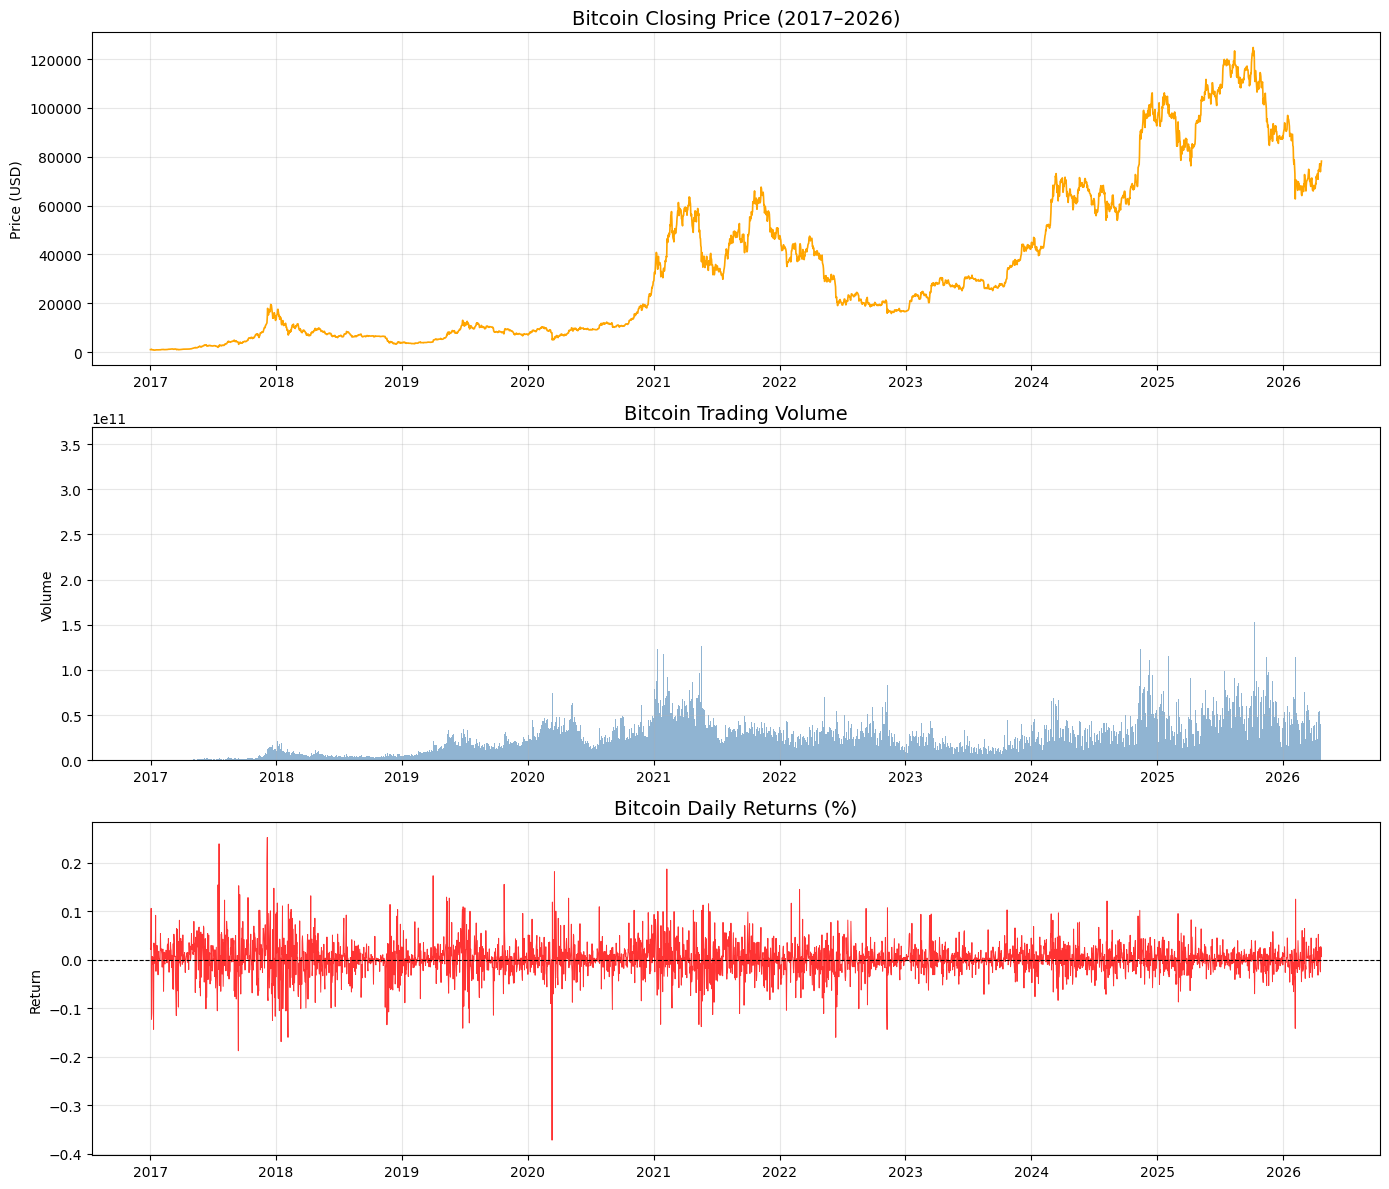
\includegraphics[width=0.95\textwidth]{fig01_eda_bitcoin.png}
\caption{Exploratory analysis of BTC-USD, 2017--2026. Top: closing price. Middle: daily trading volume. Bottom: daily percentage returns.}
\label{fig:eda}
\end{figure}

\subsection{Feature Engineering}

Seventeen \emph{stationary} features were engineered. The critical design choice --- and the principal distinction from earlier attempts at this problem --- was to avoid raw price levels as features. Raw prices are non-stationary (they trend upward by several orders of magnitude over the sample), which causes a neural network trained on prices in one regime to fail catastrophically when the test set lies in a different price range. Instead, every price-derived feature is expressed as a ratio, a rate of change, or a log-transform, all of which have approximately the same distribution throughout the sample.

\subsubsection{Target Variable: Log Return}

The target is the one-step-ahead \emph{log return}:
\begin{equation}
    r_t = \ln\!\left(\frac{C_t}{C_{t-1}}\right),
\label{eq:log-return}
\end{equation}
where $C_t$ is the closing price on day $t$. Log returns are approximately stationary, roughly symmetric around zero, and bounded by the daily price-move distribution (typically $\pm 10\%$ for BTC). Predicted log returns are converted back to USD prices at evaluation time via the identity
\begin{equation}
    \hat{C}_{t+1} = C_t \cdot \exp(\hat{r}_{t+1}).
\label{eq:price-reconstruction}
\end{equation}
For multi-step forecasts, predicted log returns are compounded recursively:
\begin{equation}
    \hat{C}_{t+h} = C_t \cdot \exp\!\left(\sum_{k=1}^{h}\hat{r}_{t+k}\right),\qquad h=1,2,3.
\label{eq:multistep-reconstruction}
\end{equation}

\subsubsection{Technical Indicators (Stationary Form)}

The following technical indicators were converted to stationary form:
\begin{itemize}[leftmargin=*]
    \item \textbf{Close-to-SMA-30 ratio:} $\mathrm{Close\_SMA30}_t = C_t / \mathrm{SMA30}_t - 1$, where $\mathrm{SMA30}$ is the 30-day simple moving average. This is the relative deviation of current price from its monthly average --- mean-reverting and scale-free.
    \item \textbf{Close-to-EMA-14 ratio:} analogously defined using the 14-day exponential moving average.
    \item \textbf{Normalized MACD:} $\mathrm{MACD}_t = (\mathrm{EMA}_{12,t} - \mathrm{EMA}_{26,t}) / C_t$. Dividing by $C_t$ removes the price-level dependence of the raw MACD.
    \item \textbf{Bollinger Band Width:} $\mathrm{BBW}_t = 2\sigma_{20,t} / \mu_{20,t}$, where $\mu_{20}$ and $\sigma_{20}$ are the 20-day rolling mean and standard deviation of Close.
    \item \textbf{Relative Strength Index (RSI-14):}
    \begin{equation}
        \mathrm{RSI}_t = 100 - \frac{100}{1 + \dfrac{\overline{\mathrm{gain}}_{14,t}}{\overline{\mathrm{loss}}_{14,t} + \epsilon}},\qquad \epsilon = 10^{-8},
        \label{eq:rsi}
    \end{equation}
    where $\overline{\mathrm{gain}}$ and $\overline{\mathrm{loss}}$ are 14-day rolling averages of positive and negative one-day price changes.
    \item \textbf{Log Volume:} $\mathrm{LogVolume}_t = \ln(1 + V_t)$, compressing the multi-order-of-magnitude range of Bitcoin trading volume.
\end{itemize}

\subsubsection{Halving-Cycle Encoding}

Bitcoin's supply issuance halves approximately every four years, a known event that has historically preceded the largest bull cycles. To let models exploit this calendar regularity, a cyclical sine-cosine encoding of days since the most recent halving is used:
\begin{equation}
    \mathrm{Halving\_sin}_t = \sin\!\left(\frac{2\pi d_t}{1460}\right), \qquad
    \mathrm{Halving\_cos}_t = \cos\!\left(\frac{2\pi d_t}{1460}\right),
\end{equation}
where $d_t$ is the number of days since the most recent of \{2012-11-28, 2016-07-09, 2020-05-11, 2024-04-19\}, and 1460 days $\approx 4$ years is the cycle length.

\subsubsection{External Features}

\textbf{Fear \& Greed Index} (0--100 integer) is used directly. \textbf{ETH, S\&P 500, Gold and Oil} are included as daily percentage returns rather than raw prices, preserving stationarity. \textbf{VIX} is already stationary and is used as a raw level. \textbf{Federal Funds Rate} and \textbf{CPI year-over-year} are used as published. The complete feature list is enumerated in Table~\ref{tab:features}.

\begin{table}[h!]
\centering
\small
\caption{Final Seventeen Stationary Features}
\label{tab:features}
\begin{tabular}{@{}clc@{}}
\toprule
\# & \textbf{Feature} & \textbf{Group} \\
\midrule
 1 & LogReturn          & technical \\
 2 & LogVolume          & technical \\
 3 & Close\_SMA30       & technical \\
 4 & Close\_EMA14       & technical \\
 5 & MACD\_norm         & technical \\
 6 & RSI\_14            & technical \\
 7 & BB\_Width          & technical \\
 8 & Halving\_sin       & technical \\
 9 & Halving\_cos       & technical \\
10 & Fear\_Greed        & sentiment \\
11 & ETH\_Return        & cross-asset \\
12 & SP500\_Return      & cross-asset \\
13 & VIX                & cross-asset \\
14 & Gold\_Return       & cross-asset \\
15 & Oil\_Return        & cross-asset \\
16 & FedFunds           & macro \\
17 & CPI\_YoY           & macro \\
\bottomrule
\end{tabular}
\end{table}

\subsection{Leak-Free Normalization}
\label{sec:leak-free}

A subtle but catastrophic error in financial deep learning is to fit feature scalers on the entire dataset before splitting into train/validation/test. This leaks information about test-period extrema (for Bitcoin, prices exceeding \$100{,}000) back into the scaler's learned minimum and maximum, allowing the model to implicitly ``know'' something about the test distribution at training time. The present pipeline deliberately avoids this by fitting the scaler only on training rows:

\begin{equation}
    \mathrm{scaler} \leftarrow \mathrm{fit}\!\left(X_{\mathrm{train}}\right),\qquad X_{\mathrm{scaled}} \leftarrow \mathrm{scaler.transform}(X).
\end{equation}

A \texttt{StandardScaler} (zero mean, unit variance) is used rather than min-max, because it is far less sensitive to extreme values and better suited to heavy-tailed financial distributions:
\begin{equation}
    z = \frac{x - \mu_{\mathrm{train}}}{\sigma_{\mathrm{train}}}.
\end{equation}
A separate target scaler is fit on the training log returns.

\subsection{Sequence Construction and Multi-Step Target}

A sliding window of $T = 60$ days produces each training sample. Each sample $\mathbf{X}_i \in \mathbb{R}^{60 \times 17}$ contains 60 days of feature vectors; the target $\mathbf{y}_i \in \mathbb{R}^{3}$ contains the next three days' scaled log returns:
\begin{equation}
    \left(\hat{r}_{t+1}, \hat{r}_{t+2}, \hat{r}_{t+3}\right)^\top = f\!\left(\mathbf{x}_{t-59}, \mathbf{x}_{t-58}, \ldots, \mathbf{x}_{t}\right).
\end{equation}
Multi-step targets discourage the model from overfitting to a single noisy horizon and produce smoother, more trend-aware predictions. Each sample also carries an \textbf{anchor} --- the most recent close price within the input window --- used at evaluation time to reconstruct absolute USD prices from log returns via Eq.~\ref{eq:multistep-reconstruction}.

\subsection{Train / Validation / Test Split}

Data is split chronologically (70\% / 15\% / 15\%), preserving temporal order. The training loader is \emph{shuffled at the sample level} because each sample is already a self-contained 60-day window; shuffling across such windows does not violate temporal causality but does break the spurious batch-level correlation that would otherwise interact poorly with BatchNorm. Validation and test loaders remain ordered.

\subsection{Evaluation Metrics}
\label{sec:metrics}

Six complementary metrics are reported for every model and every horizon $h\in\{1,2,3\}$. Let $y_i$ denote the actual price, $\hat{y}_i$ the predicted price, $N$ the number of test samples, and $a_i$ the anchor price (last close before the forecast).

\paragraph{Root Mean Squared Error (RMSE)} --- penalizes large errors more heavily:
\begin{equation}
    \mathrm{RMSE} = \sqrt{\frac{1}{N}\sum_{i=1}^{N}\left(y_i - \hat{y}_i\right)^2}.
\label{eq:rmse}
\end{equation}

\paragraph{Mean Absolute Error (MAE)}:
\begin{equation}
    \mathrm{MAE} = \frac{1}{N}\sum_{i=1}^{N}\left|y_i - \hat{y}_i\right|.
\label{eq:mae}
\end{equation}

\paragraph{Mean Absolute Percentage Error (MAPE)} --- scale-independent, enabling cross-dataset comparison:
\begin{equation}
    \mathrm{MAPE} = \frac{100}{N}\sum_{i=1}^{N}\left|\frac{y_i - \hat{y}_i}{y_i}\right|.
\label{eq:mape}
\end{equation}

\paragraph{Coefficient of Determination ($R^2$)}:
\begin{equation}
    R^2 = 1 - \frac{\sum_{i=1}^{N}\left(y_i - \hat{y}_i\right)^2}{\sum_{i=1}^{N}\left(y_i - \bar{y}\right)^2}.
\label{eq:r2}
\end{equation}

\paragraph{Directional Accuracy (DA)} --- fraction of samples whose predicted direction (up or down relative to the anchor) matches the actual direction:
\begin{equation}
    \mathrm{DA} = \frac{1}{N}\sum_{i=1}^{N} \mathbb{1}\!\left[\,(\hat{y}_i - a_i)(y_i - a_i) > 0\,\right].
\label{eq:da}
\end{equation}

\paragraph{Precision, Recall and F1 for up-moves} --- treating the prediction task as a binary up/down classification against the anchor:
\begin{equation}
    \mathrm{Precision} = \frac{TP}{TP + FP},\quad \mathrm{Recall} = \frac{TP}{TP + FN},\quad
    F_1 = 2\cdot\frac{\mathrm{Precision}\cdot\mathrm{Recall}}{\mathrm{Precision}+\mathrm{Recall}}.
\label{eq:prf1}
\end{equation}

\paragraph{Worked numerical example.} For the final test sample on horizon Day+1 produced by TCN, the anchor price was $a = \$\,77{,}971.20$. The predicted scaled log return was inverse-transformed to $\hat{r}_{+1} = -9.03\times 10^{-5}$, giving
\[
\hat{y} = a\cdot \exp(\hat{r}_{+1}) = 77{,}971.20\cdot \exp(-9.03\times 10^{-5}) \approx \$\,77{,}964.10.
\]
If the actual next-day close were, hypothetically, \$\,78{,}200, this sample would contribute $(78200 - 77964)^2 = 55{,}696$ to the RMSE numerator, $|78200-77964| = 236$ to MAE, $236/78200 \approx 0.302\%$ to MAPE, and an incorrect direction (predicted down, actual up) to DA.

\subsection{Statistical Significance: Diebold--Mariano Test}

Given two models A and B, let $e_{A,i}$ and $e_{B,i}$ denote their squared-error forecast residuals. The loss differential is $d_i = e_{A,i}^2 - e_{B,i}^2$. The DM test statistic is
\begin{equation}
    \mathrm{DM} = \frac{\bar{d}}{\sqrt{\hat{V}(\bar{d})/N}},\qquad \bar{d} = \frac{1}{N}\sum_{i=1}^{N} d_i,
\label{eq:dm}
\end{equation}
where $\hat{V}(\bar{d})$ is the Newey--West HAC variance estimator with lag $h-1$ \cite{dieboldmariano1995}. Under $H_0$ (equal forecast accuracy), DM is asymptotically standard normal. A negative DM with $p<0.05$ indicates that model A is significantly better than model B; a positive DM with $p<0.05$ indicates the reverse.

\subsection{Uncertainty Quantification: MC Dropout}

Following Gal and Ghahramani \cite{galghahramani2016}, at inference time we leave dropout layers active and perform $M = 100$ stochastic forward passes on the same input. The mean over passes is reported as the point prediction and $1.96\sigma$ as the 95\% prediction interval.

% ─────────────────────────────────────────────
\section{Proposed Solution}
% ─────────────────────────────────────────────

\subsection{System Architecture Overview}

The proposed system is a multi-model deep learning pipeline for multi-horizon Bitcoin price prediction. The pipeline consists of seven stages:
\begin{enumerate}[leftmargin=*]
    \item \textbf{Data acquisition:} live OHLCV retrieval from Yahoo Finance and external API collection.
    \item \textbf{Feature engineering:} construction of seventeen stationary features.
    \item \textbf{Preprocessing:} train-only StandardScaler fitting plus sliding-window sequence construction.
    \item \textbf{Model training:} parallel training of four architectures under identical hyperparameters.
    \item \textbf{Evaluation:} static split, walk-forward, feature-group ablation, Diebold--Mariano, MC Dropout.
    \item \textbf{Ensembling:} simple average and validation-weighted combination of the four models.
    \item \textbf{Inference:} real-time multi-step forecasting with uncertainty intervals.
\end{enumerate}

Figure~\ref{fig:pipeline-overall} depicts the end-to-end flow of these stages, showing how raw heterogeneous data sources are transformed into stationary features, processed through the leak-free normalization layer, fed in parallel to four architectures, combined via two ensemble strategies, and finally subjected to a comprehensive evaluation suite.

\begin{figure}[h!]
\centering
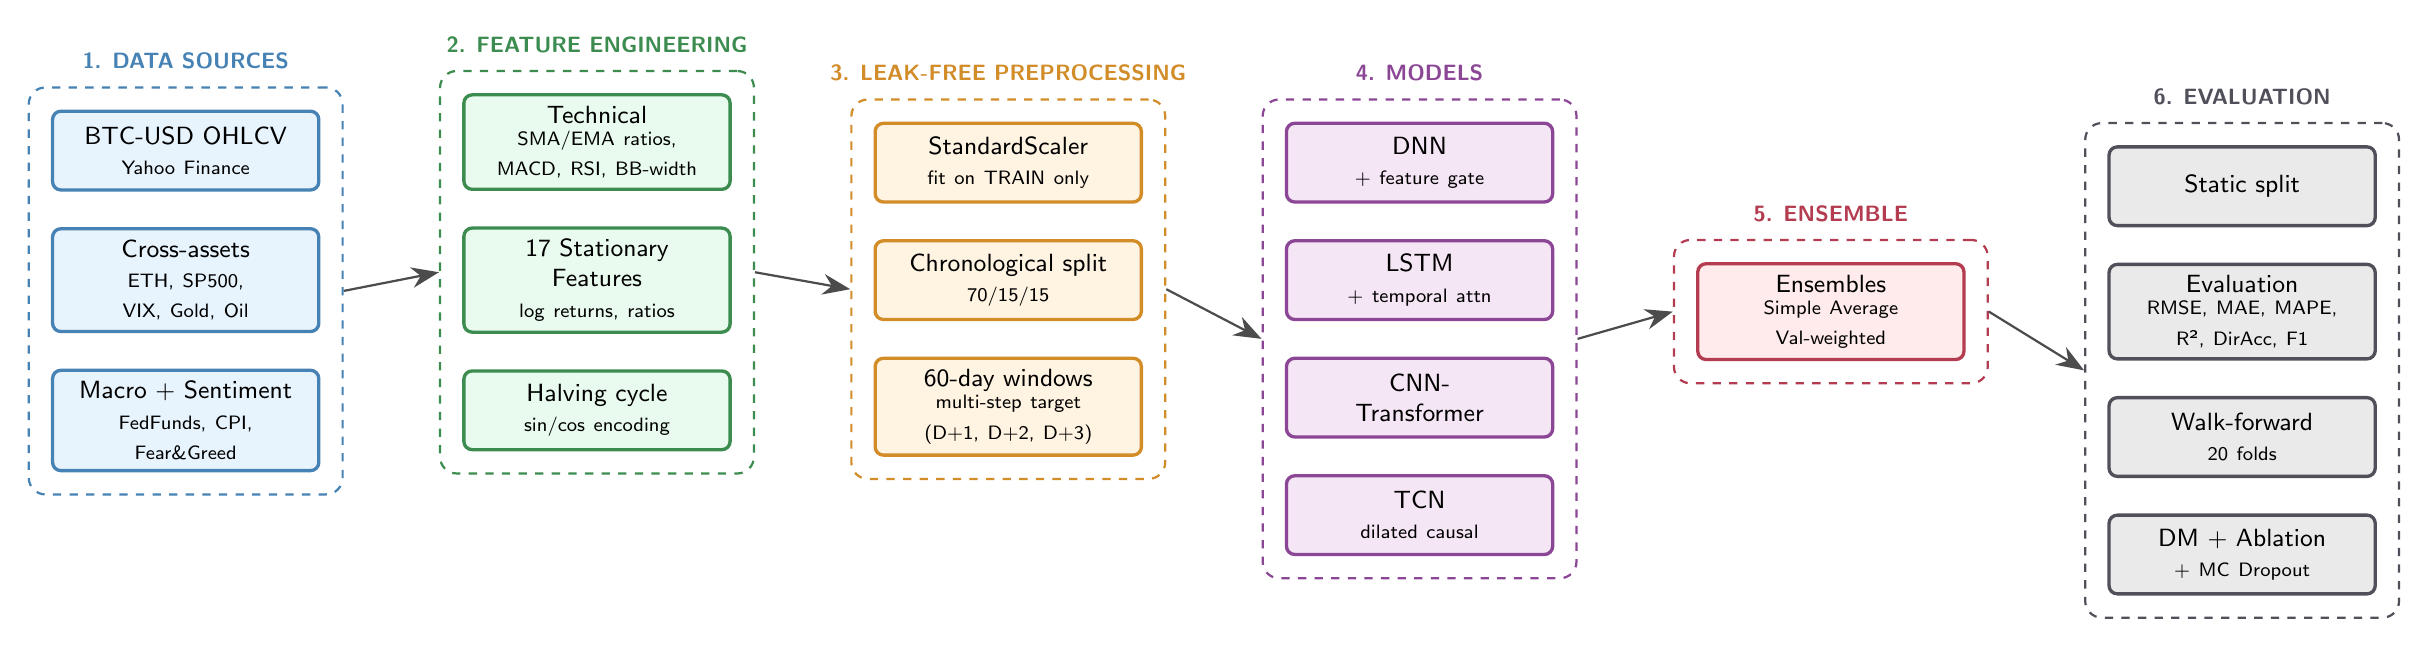
\includegraphics[width=\textwidth]{fig_pipeline_overall.png}
\caption{End-to-end pipeline overview. Six stages: (1) data sources $\to$ (2) stationary feature engineering $\to$ (3) leak-free preprocessing $\to$ (4) four parallel deep learning models $\to$ (5) two ensemble combinations $\to$ (6) comprehensive evaluation suite.}
\label{fig:pipeline-overall}
\end{figure}

\subsection{Model 1: DNN with Feature Attention Gate}

The DNN treats the flattened 60-day window as a single feature vector of dimensionality $60\times 17 = 1020$. Before flattening, a feature-attention gate computes a per-feature weight $\mathbf{g}\in[0,1]^{17}$ from the mean activation of the sequence:
\begin{equation}
    \mathbf{g} = \sigma\!\left(W_2 \cdot \mathrm{ReLU}(W_1 \cdot \bar{\mathbf{x}})\right),\qquad \bar{\mathbf{x}} = \frac{1}{60}\sum_{t=1}^{60} \mathbf{x}_t,
\end{equation}
and re-weights the input as $\mathbf{x}'_t = \mathbf{g} \odot \mathbf{x}_t$. The gated input is then processed by a four-layer MLP:
\begin{equation}
\begin{split}
    & \text{Input}(1020) \to \text{FC}(512) \to \text{BN} \to \text{ReLU} \to \text{Dropout}(0.3) \\
    & \to \text{FC}(256) \to \text{BN} \to \text{ReLU} \to \text{Dropout}(0.3) \\
    & \to \text{FC}(128) \to \text{BN} \to \text{ReLU} \to \text{Dropout}(0.2) \\
    & \to \text{FC}(64) \to \text{ReLU} \to \text{FC}(N_{\text{steps}}=3).
\end{split}
\end{equation}

The complete DNN architecture, including the feature-attention gate branch and the main MLP stack, is illustrated in Figure~\ref{fig:arch-dnn}.

\begin{figure}[h!]
\centering
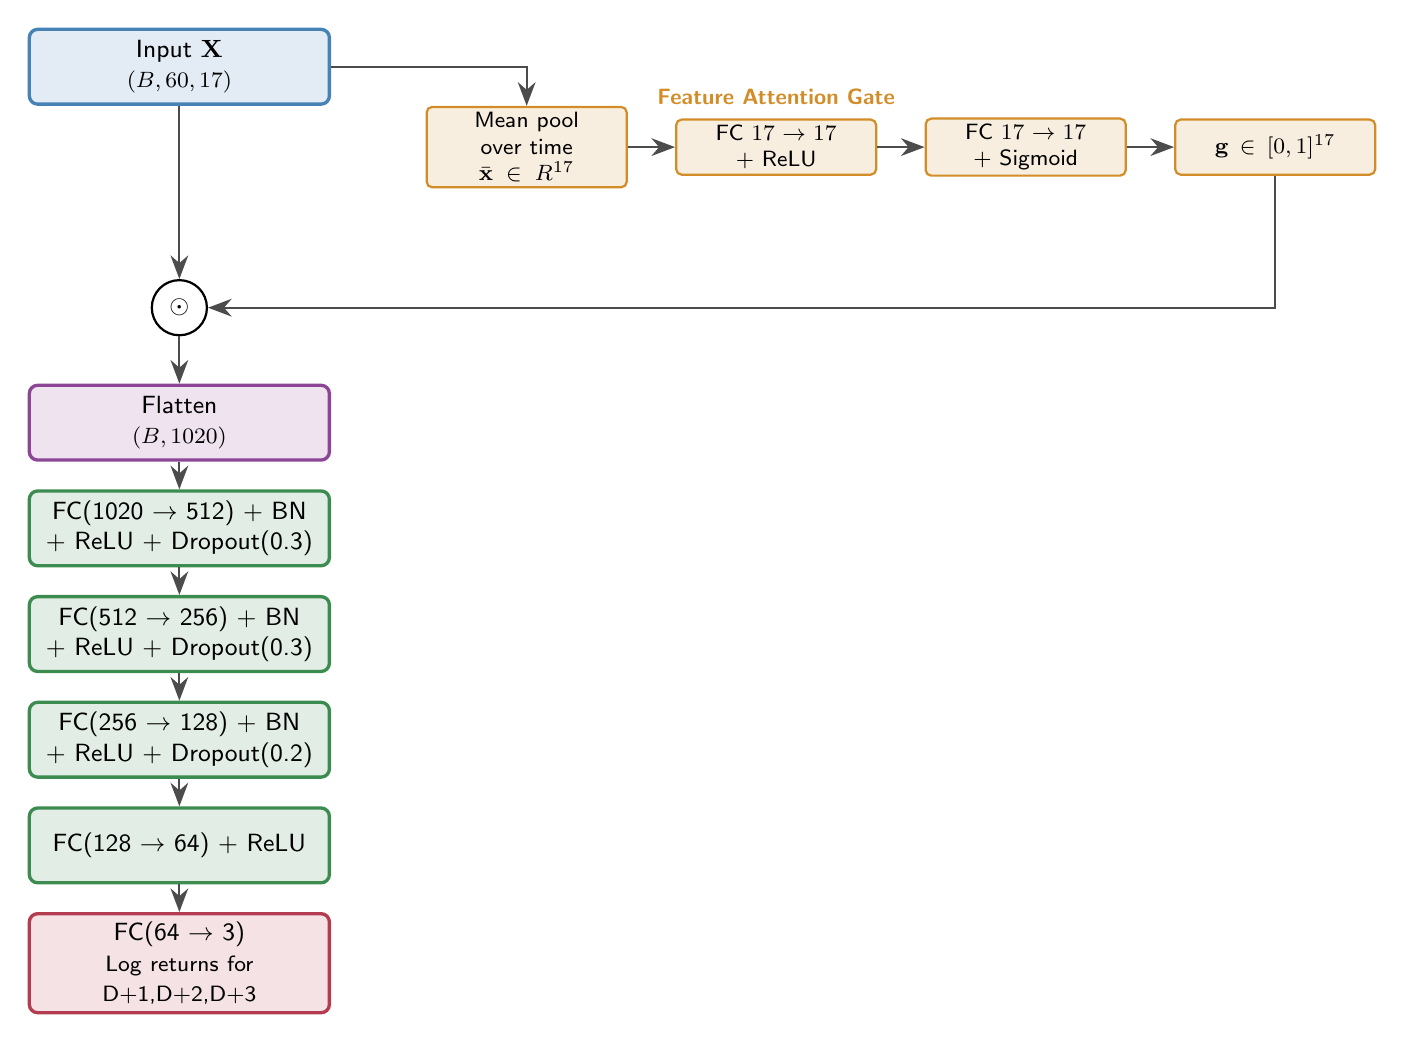
\includegraphics[width=0.78\textwidth]{fig_arch_dnn.png}
\caption{DNN architecture with feature-attention gate. The mean-pooled feature vector $\bar{\mathbf{x}}$ is passed through a small two-layer network with sigmoid output to produce the gate $\mathbf{g}$, which is then broadcast across all 60 time steps and applied element-wise to the input. The gated tensor is flattened and fed through a four-layer MLP with BatchNorm and Dropout, producing predictions for Day+1, Day+2 and Day+3.}
\label{fig:arch-dnn}
\end{figure}

\subsection{Model 2: LSTM with Temporal Self-Attention}

The LSTM model uses two stacked LSTM layers with hidden size 128 and 30\% inter-layer dropout. The canonical LSTM cell updates at each time step $t$ are
\begin{align}
    f_t &= \sigma(W_f \cdot [h_{t-1}, x_t] + b_f) \\
    i_t &= \sigma(W_i \cdot [h_{t-1}, x_t] + b_i) \\
    \tilde{c}_t &= \tanh(W_c \cdot [h_{t-1}, x_t] + b_c) \\
    c_t &= f_t \odot c_{t-1} + i_t \odot \tilde{c}_t \\
    o_t &= \sigma(W_o \cdot [h_{t-1}, x_t] + b_o) \\
    h_t &= o_t \odot \tanh(c_t).
\end{align}
Rather than using only $h_{60}$, all 60 hidden states $\{h_t\}_{t=1}^{60}$ are pooled by a learned temporal attention:
\begin{equation}
    \alpha_t = \frac{\exp(e_t)}{\sum_{s=1}^{60}\exp(e_s)},\qquad e_t = v^\top\tanh(W_a h_t),
\end{equation}
producing a context vector $\mathbf{c} = \sum_{t=1}^{60}\alpha_t h_t$ that is passed to a two-layer fully-connected head with output dimension $N_\text{steps} = 3$.

Figure~\ref{fig:arch-lstm} illustrates the unrolled LSTM, the per-step hidden states, the temporal self-attention pooling, and the prediction head. Unlike a vanilla LSTM that retains only $h_{60}$, the attention layer learns a soft weighting over all sixty hidden states, allowing the model to emphasise the time steps most informative for the upcoming forecast horizon.

\begin{figure}[h!]
\centering
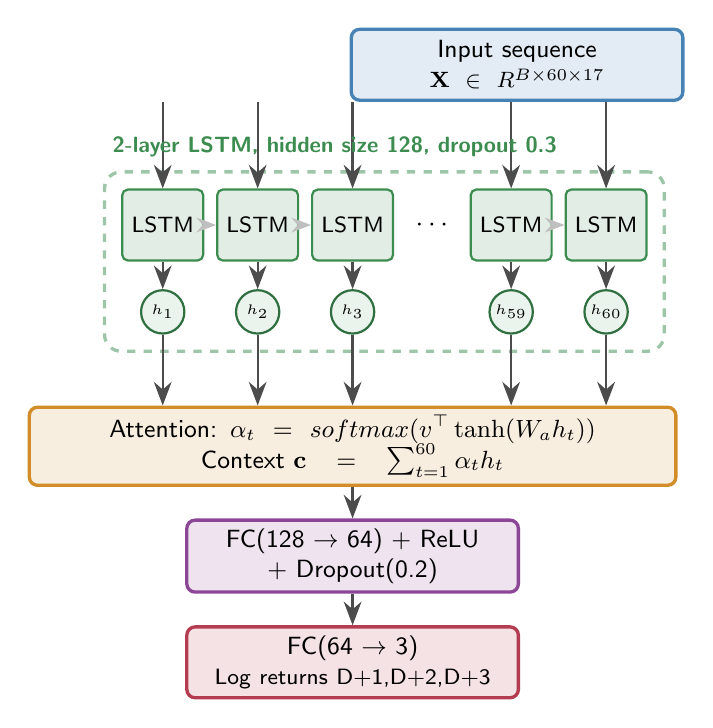
\includegraphics[width=0.85\textwidth]{fig_arch_lstm.png}
\caption{LSTM with temporal self-attention. The 60-day input is processed by two stacked LSTM layers (hidden size 128, dropout 0.3). Each hidden state $h_t$ is scored by a small attention network producing weights $\alpha_t$ that softmax to one. The context vector $\mathbf{c}$ is the weighted sum of all hidden states, then fed through a two-layer MLP head.}
\label{fig:arch-lstm}
\end{figure}

\subsection{Model 3: Hybrid CNN-Transformer}

The input is first processed by two 1D convolutional blocks (kernel size 3, channels 64 and 128) interleaved with Batch Normalization, ReLU activation, MaxPool1D (stride 2) and Dropout. MaxPooling compresses the sequence length from 60 to 30, acting as a learned downsampler. A learned positional encoding $\mathbf{P} \in \mathbb{R}^{30 \times 128}$ is added, and the result is fed to a 2-layer TransformerEncoder with 8 attention heads and feed-forward width 256. The multi-head attention at each layer computes
\begin{equation}
    \mathrm{Attention}(Q,K,V) = \mathrm{softmax}\!\left(\frac{QK^\top}{\sqrt{d_k}}\right)V,
\end{equation}
with $Q$, $K$, $V$ being learned projections of the input. A global mean pool over time followed by a two-layer MLP produces the three-horizon output.

The combined convolutional-transformer pipeline, including the multi-head attention expansion within each TransformerEncoder layer, is shown in Figure~\ref{fig:arch-cnntr}. The CNN front-end captures local short-term patterns and downsamples the sequence; the Transformer back-end captures long-range dependencies via self-attention.

\begin{figure}[h!]
\centering
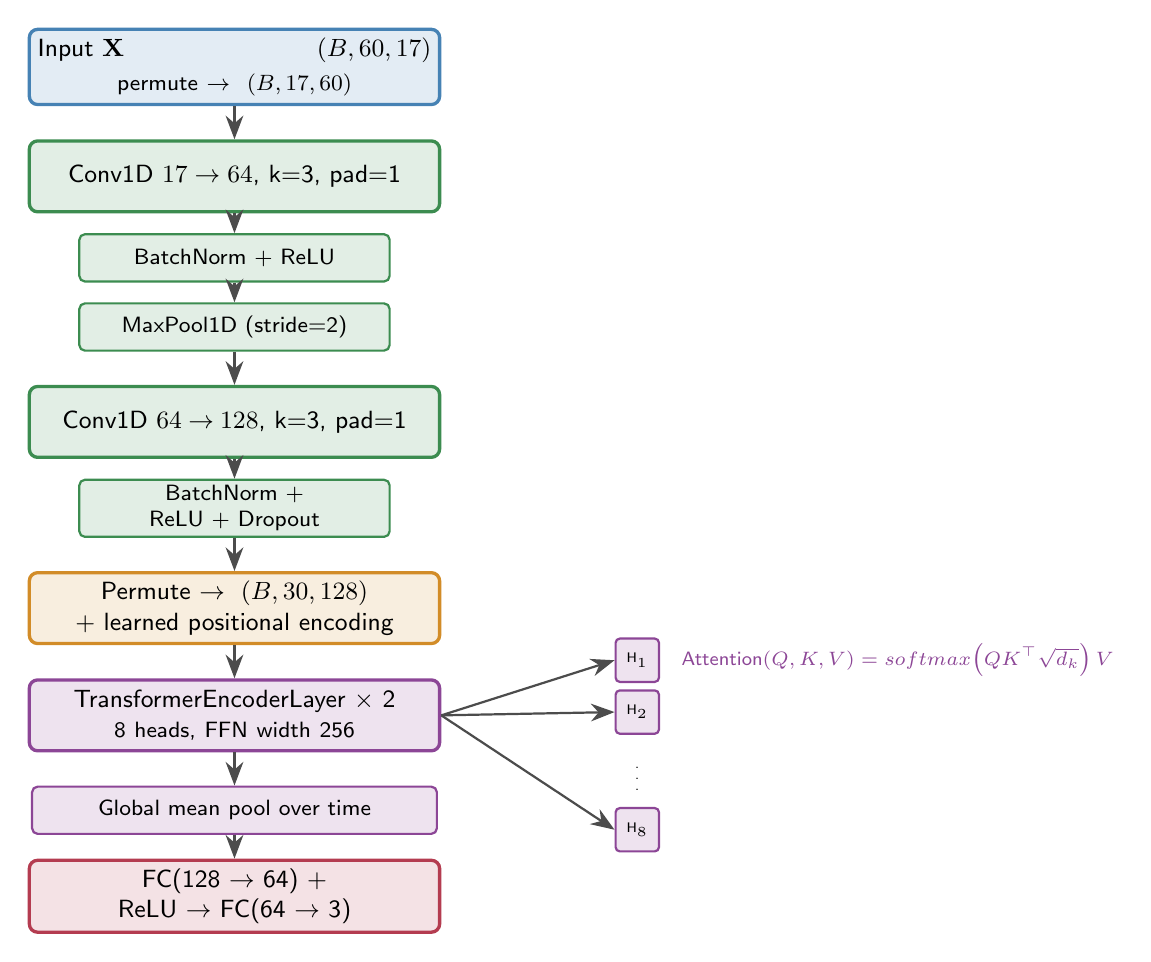
\includegraphics[width=0.7\textwidth]{fig_arch_cnntr.png}
\caption{CNN-Transformer hybrid architecture. The 60-day input is first passed through two 1D convolutional blocks with BatchNorm, ReLU and MaxPooling (stride 2), compressing the sequence length from 60 to 30. A learned positional encoding is then added before two TransformerEncoder layers with eight attention heads each. A global mean pool over the time dimension produces a fixed-size representation that is fed through a two-layer MLP head.}
\label{fig:arch-cnntr}
\end{figure}

\subsection{Model 4: Temporal Convolutional Network (TCN)}

The TCN consists of four TemporalBlock residual units. Each block applies two dilated causal convolutions (kernel size 3, weight-normalized, channels 64), each followed by a right-chomp to enforce causality, ReLU and Dropout; the block output is summed with the residual input. Dilation doubles at each block ($d_i = 2^i$ for $i=0,1,2,3$), yielding an effective receptive field of
\[
R = 1 + (3-1)(2^4 - 1) = 31\ \text{time steps}.
\]
The final time step of the final block's output passes through a two-layer MLP to produce the three-horizon prediction. Compared to recurrent models, the TCN is fully parallelizable in the time dimension and immune to the vanishing/exploding-gradient issues that plague deep RNNs \cite{bai2018tcn,jin2025tcn}.

The full TCN structure --- the four-block stack on the left, with the internal layout of a single TemporalBlock (dilated causal convolution, chomp, ReLU, dropout, and residual skip) on the right --- is shown in Figure~\ref{fig:arch-tcn}.

\begin{figure}[h!]
\centering
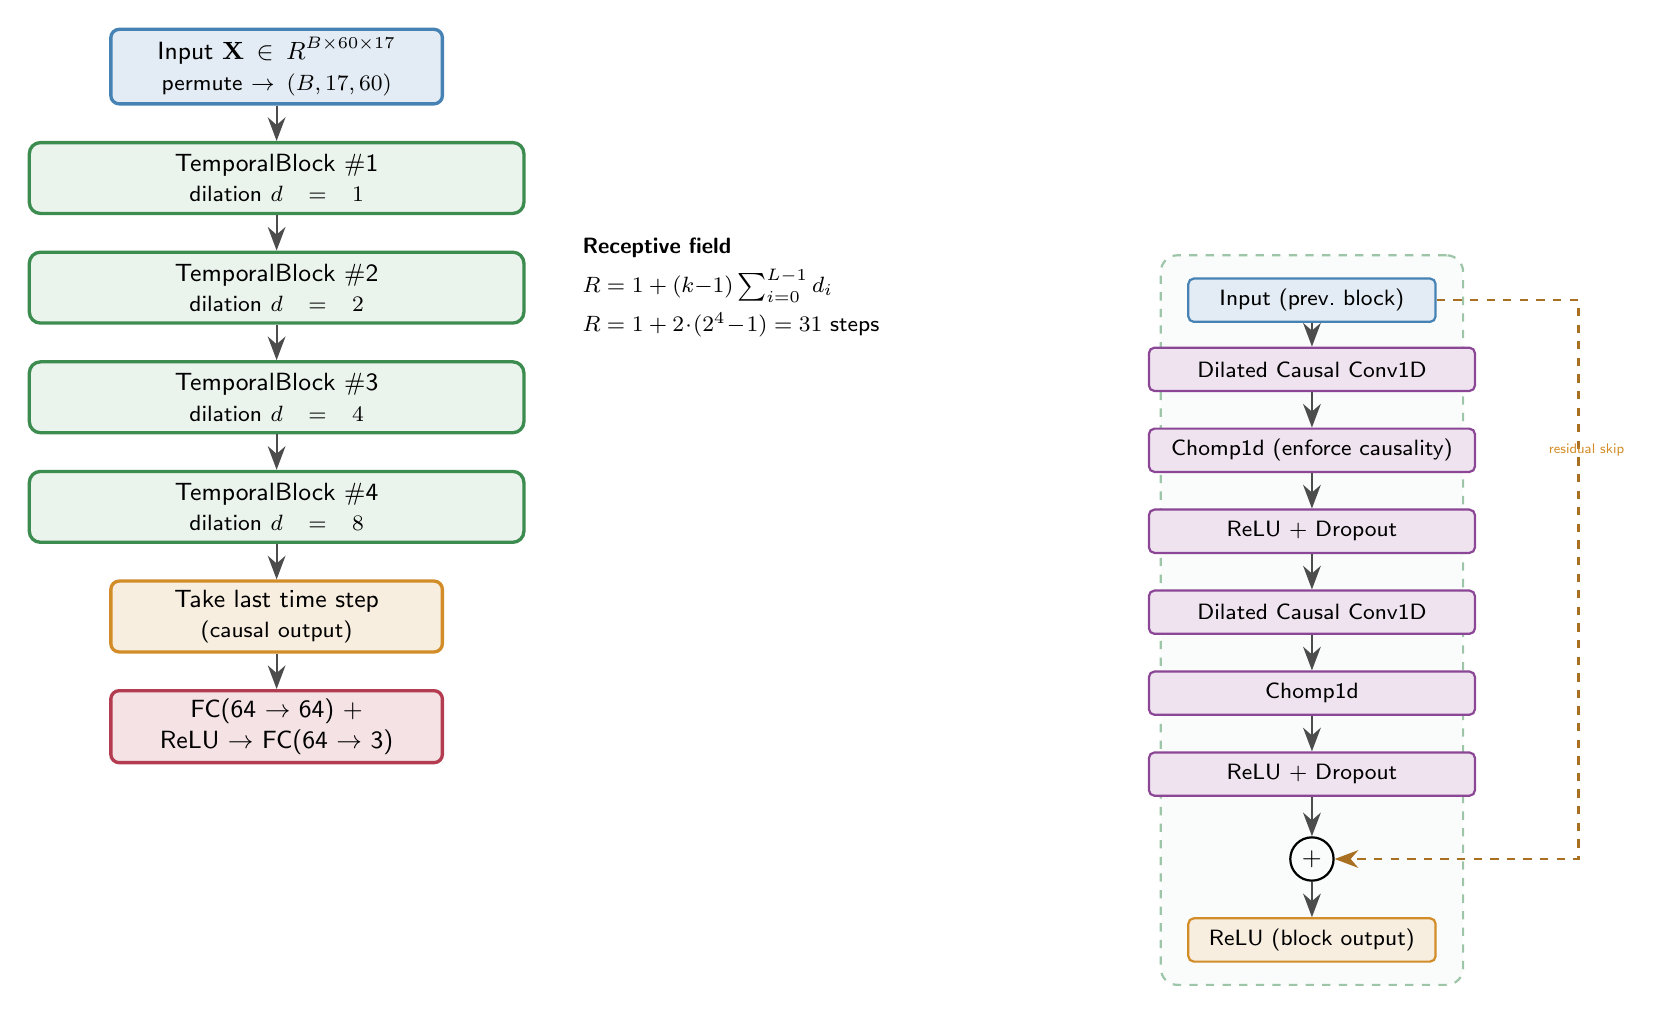
\includegraphics[width=\textwidth]{fig_arch_tcn.png}
\caption{Temporal Convolutional Network architecture. \textbf{Left:} the main chain --- four TemporalBlocks with dilation factors $d \in \{1, 2, 4, 8\}$, ending with a final-time-step extraction and a two-layer MLP head. \textbf{Right:} the internal structure of one TemporalBlock --- two dilated causal convolutions, each followed by Chomp1d (which removes the right-side padding to enforce causality), ReLU and dropout, with a residual skip connection that bypasses both convolutions. The receptive field at the output is $R = 1 + (k-1)(2^L - 1) = 31$ time steps.}
\label{fig:arch-tcn}
\end{figure}

\subsection{Training Strategy}

All four models share an identical training protocol:
\begin{itemize}[leftmargin=*]
    \item \textbf{Optimizer:} AdamW with learning rate $10^{-3}$ and weight decay $10^{-4}$.
    \item \textbf{Loss function:} Huber loss (Smooth-L1) with $\delta = 1$:
    \begin{equation}
        \mathcal{L}_\mathrm{Huber}(y,\hat{y}) =
        \begin{cases}
            \frac{1}{2}(y - \hat{y})^2 & \text{if } |y - \hat{y}| \leq \delta \\
            \delta(|y - \hat{y}| - \tfrac{1}{2}\delta) & \text{otherwise}.
        \end{cases}
        \label{eq:huber}
    \end{equation}
    Huber loss is quadratic for small residuals (preserving smooth gradients) but linear for large residuals, so isolated extreme-move days do not dominate the gradient --- crucial for a heavy-tailed asset like Bitcoin \cite{jin2025tcn}.
    \item \textbf{Learning rate schedule:} Cosine annealing over 100 epochs.
    \item \textbf{Batch size:} 64.
    \item \textbf{Early stopping:} patience of 15 epochs on validation loss; best weights are restored.
    \item \textbf{Gradient clipping:} global norm capped at 1.0.
\end{itemize}

\subsection{Ensembling Strategy}

Two ensembles are constructed, both using only validation-set information (never test):

\textbf{Simple Average.} The mean of the four models' scaled log-return predictions.

\textbf{Weighted by Validation MAPE.} The weight for model $m$ is the inverse of its Day+1 validation MAPE, normalized:
\begin{equation}
    w_m = \frac{1/\mathrm{MAPE}^{\mathrm{val}}_m}{\sum_{m'}1/\mathrm{MAPE}^{\mathrm{val}}_{m'}}.
\end{equation}
This differs from the CFA approach of Wu et al.\ \cite{wu2025cfa} in two important ways: (i) weights are locked in using validation data only, never test; and (ii) there is no per-day oracle selection across combination strategies.

Figure~\ref{fig:ensemble} illustrates the full ensemble pipeline: each of the four models produces a scaled log-return prediction $\hat{\mathbf{r}}_m$, the four predictions are combined by a simple average and by a validation-MAPE-weighted average, and the resulting ensemble outputs are converted back to USD prices via the same compounding identity used for individual models.

\begin{figure}[h!]
\centering
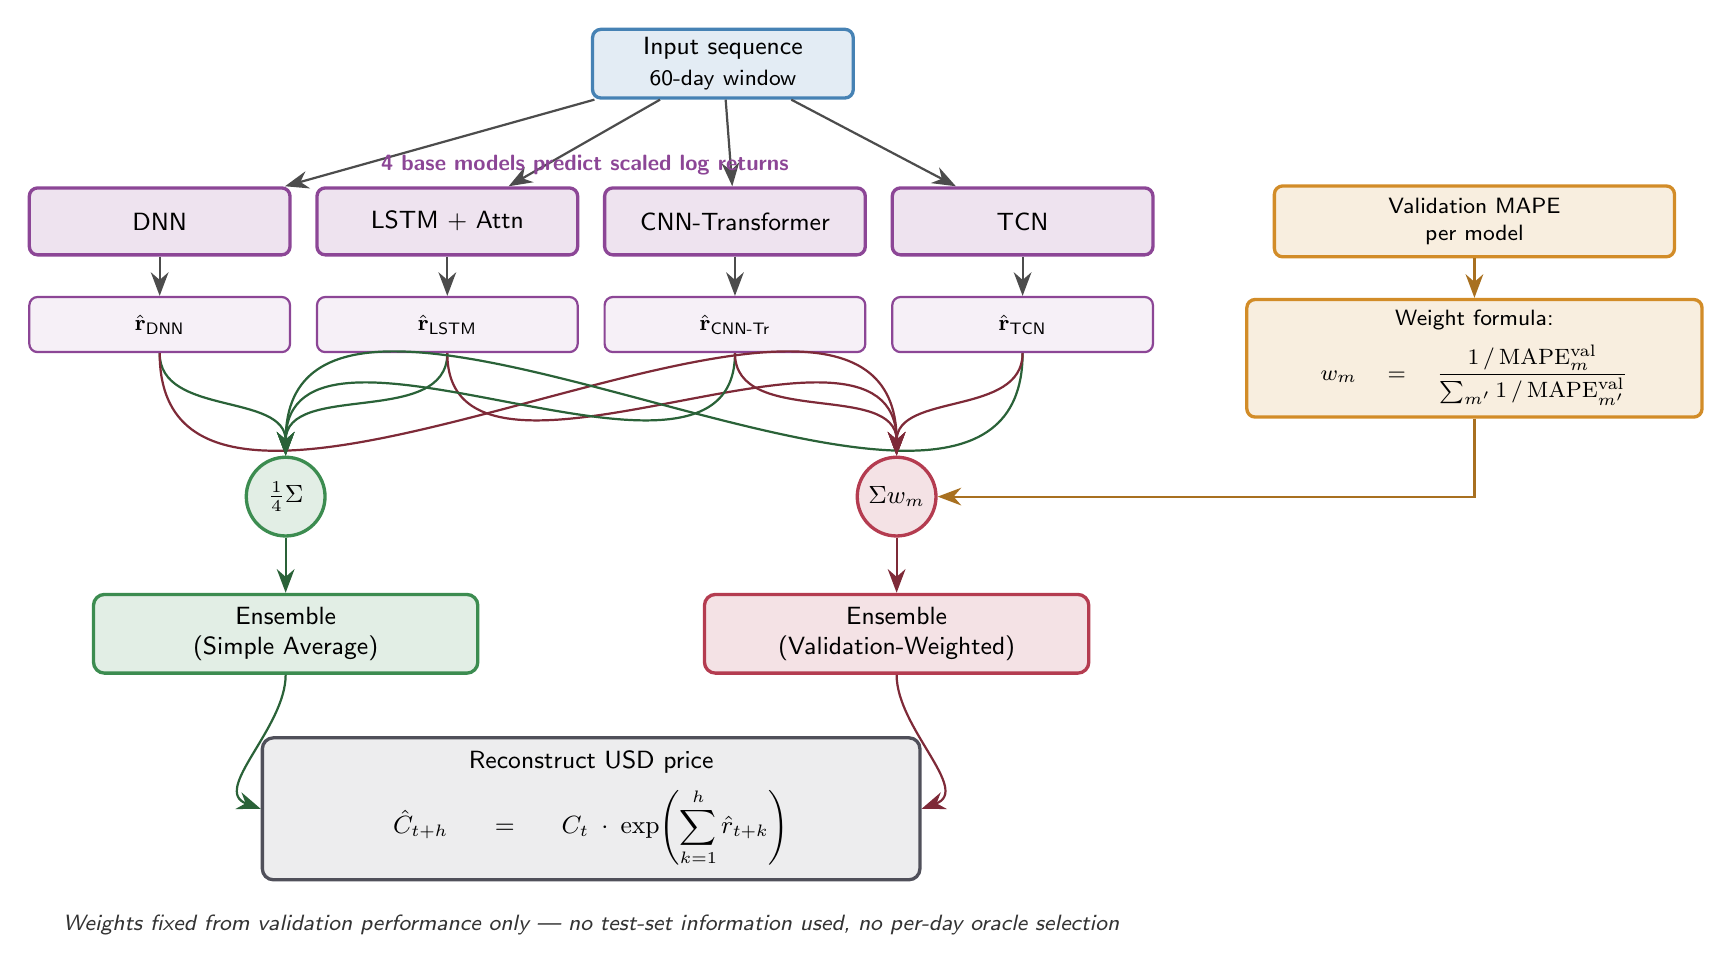
\includegraphics[width=\textwidth]{fig_ensemble.png}
\caption{Ensemble pipeline. The same 60-day input sequence is fed to all four base models. Each model produces a scaled log-return vector $\hat{\mathbf{r}}_m$ for horizons Day+1, Day+2 and Day+3. Two ensembles are then computed in parallel: a simple average (left, green) and a validation-weighted average (right, red), where weights are derived from per-model validation-set MAPE. The ensemble outputs go through the same price-reconstruction step $\hat{C}_{t+h} = C_t \cdot \exp(\sum_{k=1}^{h}\hat{r}_{t+k})$ used for individual model predictions. Critically, ensemble weights are fixed using validation data only --- no test-set information is used and there is no per-day oracle selection.}
\label{fig:ensemble}
\end{figure}

% ─────────────────────────────────────────────
\section{Implementation}
% ─────────────────────────────────────────────

\subsection{Software Environment}

The project was implemented in Python 3.10+ with PyTorch 2.x, executed on a CUDA-capable GPU when available. Key libraries: \texttt{yfinance}, \texttt{pytrends}, \texttt{transformers}, \texttt{pandas}, \texttt{numpy}, \texttt{scikit-learn}, \texttt{scipy} (for the Diebold--Mariano test), and \texttt{matplotlib}/\texttt{seaborn} for visualization. All random seeds are fixed (NumPy and PyTorch) for reproducibility.

\subsection{Sequence and Anchor Construction}

\begin{lstlisting}[language=Python, caption=Multi-step sequence construction with anchor prices]
def create_sequences_returns(feat_data, target_data, close_raw,
                             seq_len, n_steps):
    X, y, anchors = [], [], []
    for i in range(seq_len, len(feat_data) - n_steps + 1):
        X.append(feat_data[i - seq_len : i])
        y.append(target_data[i : i + n_steps, 0])
        anchors.append(close_raw[i - 1])   # last close in input window
    return np.array(X), np.array(y), np.array(anchors)
\end{lstlisting}

\subsection{DNN with Feature Attention Gate}

\begin{lstlisting}[language=Python, caption=DNN architecture with feature gating]
class DeepNeuralNetwork(nn.Module):
    def __init__(self, input_dim, num_features, n_steps=1):
        super().__init__()
        self.feature_gate = nn.Sequential(
            nn.Linear(num_features, num_features), nn.ReLU(),
            nn.Linear(num_features, num_features), nn.Sigmoid())
        self.model = nn.Sequential(
            nn.Flatten(),
            nn.Linear(input_dim, 512), nn.BatchNorm1d(512),
            nn.ReLU(), nn.Dropout(0.3),
            nn.Linear(512, 256), nn.BatchNorm1d(256),
            nn.ReLU(), nn.Dropout(0.3),
            nn.Linear(256, 128), nn.BatchNorm1d(128),
            nn.ReLU(), nn.Dropout(0.2),
            nn.Linear(128, 64), nn.ReLU(),
            nn.Linear(64, n_steps))
    def forward(self, x):
        gate = self.feature_gate(x.mean(dim=1))   # (B, F)
        x = x * gate.unsqueeze(1)                  # broadcast over time
        return self.model(x)
\end{lstlisting}

\subsection{LSTM with Temporal Self-Attention}

\begin{lstlisting}[language=Python, caption=LSTM + temporal self-attention]
class LSTMAttentionModel(nn.Module):
    def __init__(self, input_size, hidden_size=128, num_layers=2,
                 dropout=0.3, n_steps=1):
        super().__init__()
        self.lstm = nn.LSTM(input_size, hidden_size, num_layers,
                            dropout=dropout, batch_first=True)
        self.attention = nn.Sequential(
            nn.Linear(hidden_size, hidden_size//2), nn.Tanh(),
            nn.Linear(hidden_size//2, 1))
        self.fc = nn.Sequential(
            nn.Linear(hidden_size, 64), nn.ReLU(),
            nn.Dropout(0.2), nn.Linear(64, n_steps))
    def forward(self, x):
        lstm_out, _  = self.lstm(x)
        scores  = self.attention(lstm_out)
        weights = torch.softmax(scores, dim=1)
        context = (lstm_out * weights).sum(dim=1)
        return self.fc(context)
\end{lstlisting}

\subsection{CNN-Transformer Hybrid}

\begin{lstlisting}[language=Python, caption=CNN-Transformer hybrid]
class CNNTransformerModel(nn.Module):
    def __init__(self, input_size, seq_len, d_model=128,
                 nhead=8, num_tf_layers=2, dropout=0.3, n_steps=1):
        super().__init__()
        self.cnn = nn.Sequential(
            nn.Conv1d(input_size, 64, 3, padding=1),
            nn.BatchNorm1d(64), nn.ReLU(), nn.MaxPool1d(2),
            nn.Conv1d(64, d_model, 3, padding=1),
            nn.BatchNorm1d(d_model), nn.ReLU(), nn.Dropout(dropout))
        self.pos_encoding = nn.Parameter(
            torch.randn(1, seq_len//2, d_model) * 0.02)
        encoder_layer = nn.TransformerEncoderLayer(
            d_model=d_model, nhead=nhead,
            dim_feedforward=256, dropout=dropout, batch_first=True)
        self.transformer = nn.TransformerEncoder(encoder_layer,
                                                 num_layers=num_tf_layers)
        self.fc = nn.Sequential(
            nn.Linear(d_model, 64), nn.ReLU(),
            nn.Dropout(0.2), nn.Linear(64, n_steps))
    def forward(self, x):
        x = x.permute(0, 2, 1)        # to (B, F, T) for Conv1d
        x = self.cnn(x)
        x = x.permute(0, 2, 1)        # back to (B, T', d_model)
        x = x + self.pos_encoding[:, :x.size(1), :]
        x = self.transformer(x)
        return self.fc(x.mean(dim=1))
\end{lstlisting}

\subsection{Temporal Convolutional Network}

\begin{lstlisting}[language=Python, caption=TCN with dilated causal convolutions and residual blocks]
class Chomp1d(nn.Module):
    def __init__(self, chomp): super().__init__(); self.chomp = chomp
    def forward(self, x): return x[:, :, :-self.chomp].contiguous()

class TemporalBlock(nn.Module):
    def __init__(self, n_in, n_out, k, dilation, padding, dropout=0.2):
        super().__init__()
        self.net = nn.Sequential(
            nn.utils.weight_norm(nn.Conv1d(n_in, n_out, k,
                padding=padding, dilation=dilation)),
            Chomp1d(padding), nn.ReLU(), nn.Dropout(dropout),
            nn.utils.weight_norm(nn.Conv1d(n_out, n_out, k,
                padding=padding, dilation=dilation)),
            Chomp1d(padding), nn.ReLU(), nn.Dropout(dropout))
        self.downsample = (nn.Conv1d(n_in, n_out, 1)
                           if n_in != n_out else None)
        self.relu_out = nn.ReLU()
    def forward(self, x):
        out = self.net(x)
        res = x if self.downsample is None else self.downsample(x)
        return self.relu_out(out + res)

class TCN(nn.Module):
    def __init__(self, input_size, num_channels=(64,64,64,64),
                 kernel_size=3, dropout=0.2, n_steps=1):
        super().__init__()
        blocks = []
        for i, out_ch in enumerate(num_channels):
            d = 2**i; in_ch = input_size if i==0 else num_channels[i-1]
            blocks.append(TemporalBlock(in_ch, out_ch, kernel_size, d,
                (kernel_size-1)*d, dropout))
        self.tcn = nn.Sequential(*blocks)
        self.fc  = nn.Sequential(
            nn.Linear(num_channels[-1], 64), nn.ReLU(),
            nn.Dropout(0.2), nn.Linear(64, n_steps))
    def forward(self, x):
        x = x.permute(0, 2, 1)        # (B, F, T)
        x = self.tcn(x)
        return self.fc(x[:, :, -1])   # last time step (causal)
\end{lstlisting}

\subsection{Training Loop with AdamW + Huber}

\begin{lstlisting}[language=Python, caption={Training loop with cosine schedule, Huber loss and early stopping}]
def train_model(model, train_loader, val_loader, epochs=100,
                lr=1e-3, patience=15):
    model.to(device)
    opt   = torch.optim.AdamW(model.parameters(), lr=lr, weight_decay=1e-4)
    sched = torch.optim.lr_scheduler.CosineAnnealingLR(opt, T_max=epochs)
    crit  = nn.HuberLoss(delta=1.0)
    best, patience_ctr = float('inf'), 0
    for epoch in range(1, epochs+1):
        model.train()
        for Xb, yb in train_loader:
            Xb, yb = Xb.to(device), yb.to(device)
            opt.zero_grad()
            loss = crit(model(Xb), yb); loss.backward()
            nn.utils.clip_grad_norm_(model.parameters(), 1.0)
            opt.step()
        # ...validation, early stopping, best-weight restoration...
        sched.step()
\end{lstlisting}

\subsection{Walk-Forward Validation}

Walk-forward validation re-trains the model on an expanding window and evaluates on the subsequent month. Parameters: $\mathrm{INIT\_TRAIN\_MONTHS}=24$, $\mathrm{STEP\_MONTHS}=4$, $\mathrm{EVAL\_MONTHS}=1$, $\mathrm{WF\_EPOCHS}=5$. This yields twenty folds covering April 2019 through August 2025.

\subsection{Real-Time Inference Pipeline}

After training, the four models are serialized via \texttt{torch.save(model.state\_dict(), ...)}. The inference pipeline fetches the most recent 150 days of live BTC-USD data, re-engineers the seventeen features using the exact same transformations and the same fitted scalers (transform only, no re-fitting), constructs the trailing 60-day sequence, and runs all four models plus both ensembles. For the CNN-Transformer model, MC Dropout is invoked to produce a 95\% prediction interval. Outputs are rendered as a prediction table, a multi-step forecast chart, and a historical context plot.

% ─────────────────────────────────────────────
\section{Evaluation}
% ─────────────────────────────────────────────

\subsection{Training Dynamics}

Under the unified training protocol (AdamW, Huber loss, cosine annealing), all four models early-stopped between epochs 20 and 30 as validation loss plateaued. Because the target is the \emph{log return}, validation loss stabilizes at a small positive value rather than decreasing indefinitely --- log returns are largely unpredictable, so fitting validation loss to zero would require memorizing noise. This is healthy behaviour and indicates that the models have learned what is learnable without overfitting.

Figure~\ref{fig:loss-curves} shows the training and validation loss curves for all four architectures. The near-parallel tracking of train and validation loss, together with early stopping before any divergence, confirms that regularization (dropout, weight decay, gradient clipping, cosine LR) is effectively suppressing overfitting across all four architectures.

\begin{figure}[h!]
\centering
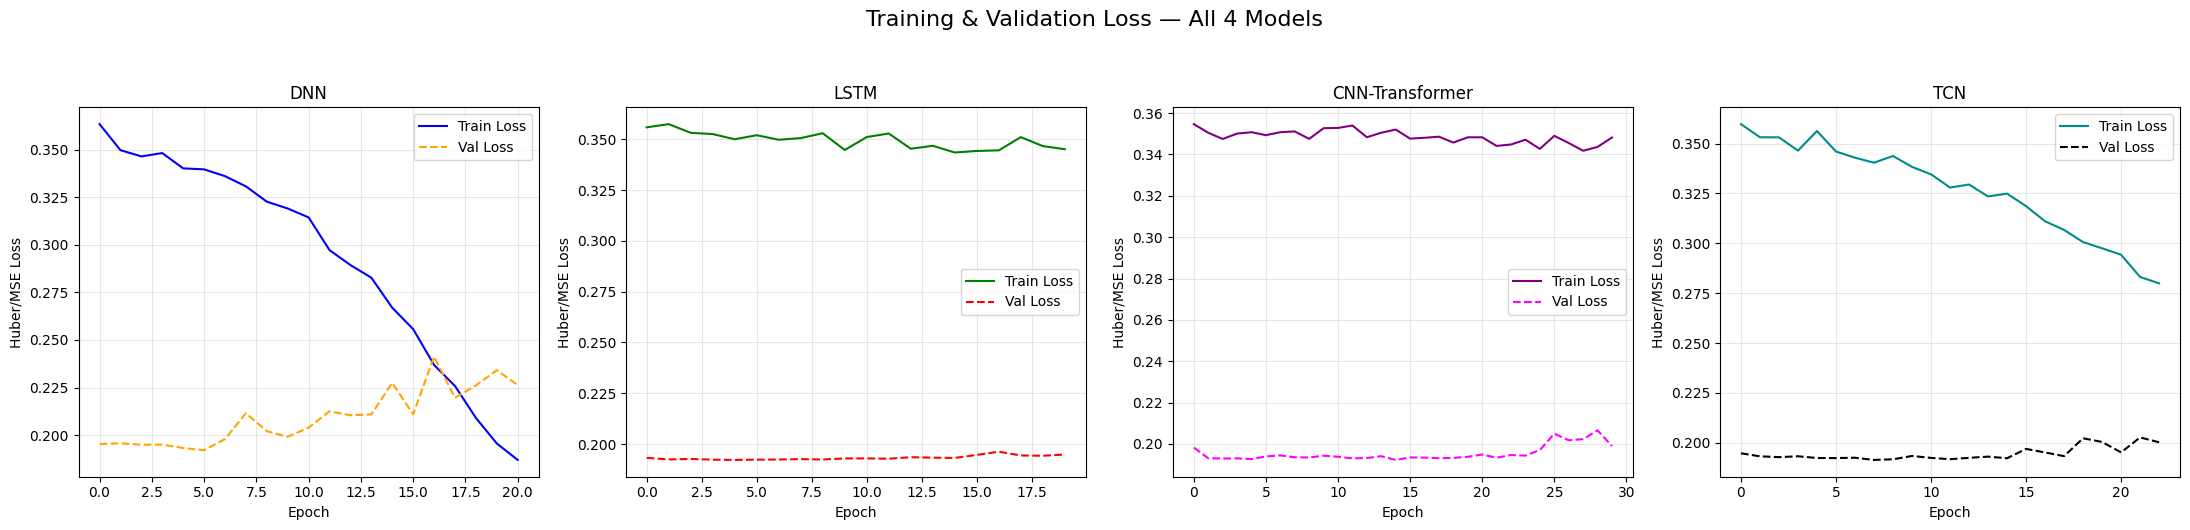
\includegraphics[width=0.95\textwidth]{fig02_loss_curves.png}
\caption{Training and validation Huber-loss curves for the four models under identical training hyperparameters.}
\label{fig:loss-curves}
\end{figure}

\subsection{Naive Random-Walk Baseline}

Before comparing models, the na\"ive random-walk baseline --- predicting ``tomorrow's price equals today's'' --- is computed on the static test set (Table~\ref{tab:naive}). This is the first legitimate comparison any daily BTC forecast must pass.

\begin{table}[h!]
\centering
\small
\caption{Na\"ive Random-Walk Baseline (Test Set)}
\label{tab:naive}
\begin{tabular}{@{}lcccc@{}}
\toprule
\textbf{Horizon} & \textbf{RMSE (\$)} & \textbf{MAE (\$)} & \textbf{MAPE (\%)} & \textbf{$R^2$} \\
\midrule
Day+1 & 2{,}152 & 1{,}557 & 1.682 & 0.9806 \\
Day+2 & 2{,}950 & 2{,}223 & 2.396 & 0.9636 \\
Day+3 & 3{,}534 & 2{,}714 & 2.925 & 0.9479 \\
\bottomrule
\end{tabular}
\end{table}

\subsection{Static-Split Test Performance}

Table~\ref{tab:results} reports per-horizon metrics for every model on the held-out test period.

\begin{table}[h!]
\centering
\small
\caption{Per-Horizon Test Performance (Static 70/15/15 Split)}
\label{tab:results}
\begin{tabular}{@{}llccccc@{}}
\toprule
\textbf{Model} & \textbf{Horizon} & \textbf{RMSE (\$)} & \textbf{MAE (\$)} & \textbf{MAPE (\%)} & \textbf{$R^2$} & \textbf{DirAcc} \\
\midrule
\multirow{3}{*}{DNN}             & Day+1 & 2{,}168 & 1{,}583 & 1.711 & 0.9803 & 0.501 \\
                                 & Day+2 & 3{,}002 & 2{,}269 & 2.448 & 0.9623 & 0.513 \\
                                 & Day+3 & 3{,}612 & 2{,}744 & 2.958 & 0.9456 & 0.521 \\
\midrule
\multirow{3}{*}{LSTM}            & Day+1 & 2{,}154 & 1{,}565 & 1.690 & 0.9805 & 0.503 \\
                                 & Day+2 & 2{,}955 & 2{,}241 & 2.415 & 0.9635 & 0.497 \\
                                 & Day+3 & 3{,}542 & 2{,}718 & 2.932 & 0.9476 & 0.531 \\
\midrule
\multirow{3}{*}{CNN-Transformer} & Day+1 & 2{,}182 & 1{,}605 & 1.733 & 0.9800 & 0.513 \\
                                 & Day+2 & 3{,}058 & 2{,}349 & 2.530 & 0.9609 & 0.503 \\
                                 & Day+3 & 3{,}723 & 2{,}908 & 3.128 & 0.9421 & 0.511 \\
\midrule
\multirow{3}{*}{TCN}             & Day+1 & \textbf{2{,}144} & 1{,}571 & 1.693 & \textbf{0.9807} & 0.505 \\
                                 & Day+2 & 2{,}950 & 2{,}236 & 2.405 & 0.9636 & 0.531 \\
                                 & Day+3 & 3{,}543 & 2{,}725 & 2.926 & 0.9476 & \textbf{0.535} \\
\midrule
\multirow{3}{*}{Ensemble (Avg)}  & Day+1 & 2{,}146 & \textbf{1{,}561} & \textbf{1.687} & 0.9807 & 0.507 \\
                                 & Day+2 & 2{,}952 & 2{,}240 & 2.415 & 0.9636 & 0.525 \\
                                 & Day+3 & 3{,}533 & 2{,}703 & 2.912 & 0.9479 & 0.551 \\
\midrule
\multirow{3}{*}{Ensemble (Wtd)}  & Day+1 & 2{,}146 & 1{,}561 & 1.687 & 0.9807 & 0.505 \\
                                 & Day+2 & 2{,}951 & 2{,}240 & 2.415 & 0.9636 & 0.523 \\
                                 & Day+3 & 3{,}533 & 2{,}703 & 2.913 & 0.9479 & 0.551 \\
\bottomrule
\end{tabular}
\end{table}

\noindent\textbf{Honest interpretation.} Every model is within \$40 of the na\"ive baseline on Day+1 RMSE, and the spread among models is roughly \$40 overall. The test period happens to coincide with a persistent upward trend during which ``tomorrow $=$ today'' is already a strong heuristic, so the scope for any model to \emph{substantially} outperform the baseline is small. What the static split does confirm is that every model has successfully learned a mapping from inputs to future log returns that does not embarrassingly underperform the na\"ive predictor --- which, given that the predecessor version of this project produced $R^2$ values between $-5$ and $-17$ on the same data, is a meaningful milestone.

Figures~\ref{fig:predictions} and~\ref{fig:model-comparison} visualize the test-set predictions and the per-metric model comparison respectively. In Figure~\ref{fig:predictions}, all four model trajectories lie visually on top of the actual-price curve --- consistent with the near-identical metrics in Table~\ref{tab:results}. Figure~\ref{fig:model-comparison} makes the narrowness of the between-model gap explicit: the TCN and the ensembles share the lowest RMSE/MAE bars, while the CNN-Transformer is a small but visible step behind.

\begin{figure}[h!]
\centering
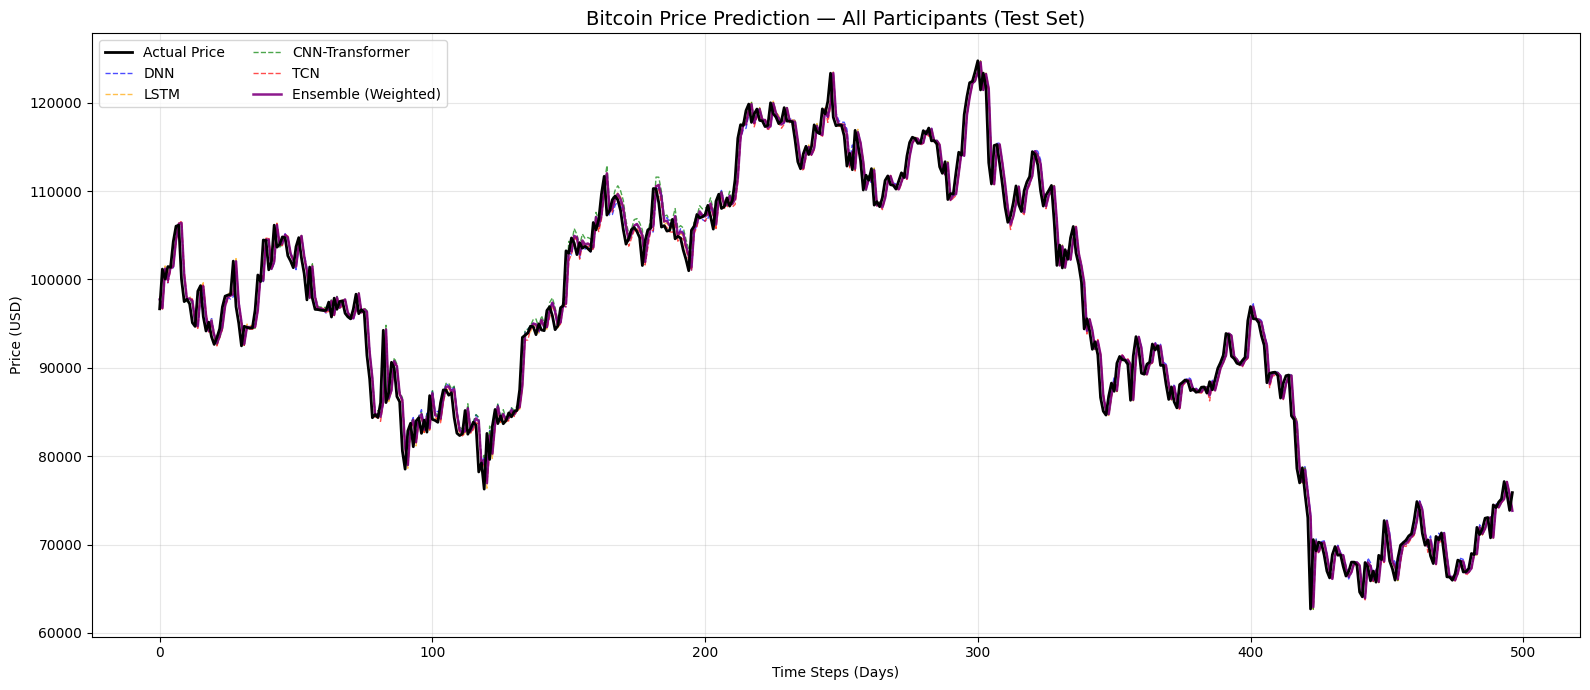
\includegraphics[width=0.95\textwidth]{fig03_predictions_vs_actual.png}
\caption{Day+1 test-set predictions vs.\ actual BTC closing prices for the four models. All trajectories are visually indistinguishable from the actual-price line at chart scale.}
\label{fig:predictions}
\end{figure}

\begin{figure}[h!]
\centering
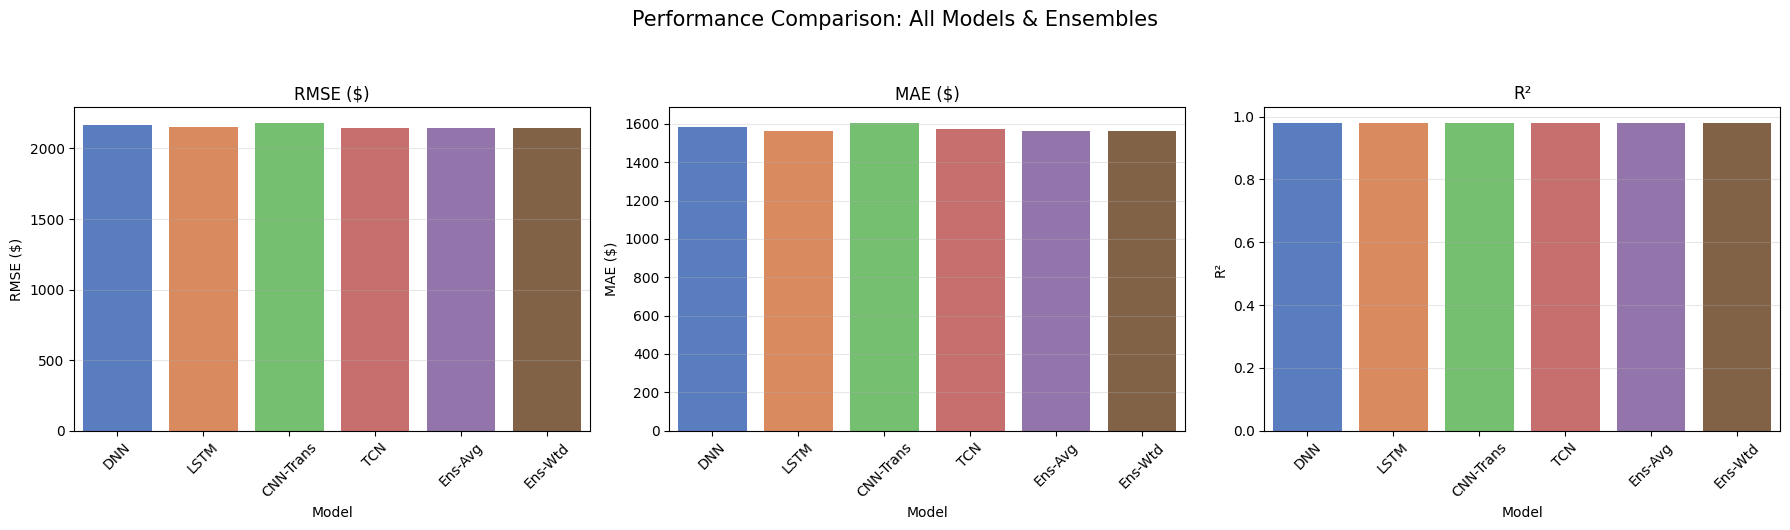
\includegraphics[width=0.95\textwidth]{fig04_model_comparison.png}
\caption{Bar-chart comparison of the four architectures on RMSE, MAE and $R^2$ (Day+1 test-set metrics).}
\label{fig:model-comparison}
\end{figure}

\subsection{Walk-Forward Validation}

Walk-forward validation is a more demanding test, re-training the model on an expanding window and evaluating on the subsequent month. It averages over twenty different one-month test periods spanning different market regimes (pre-pandemic, COVID-era, 2021 bull run, 2022 crash, 2023--24 recovery, 2024--25 rally). The per-fold results for LSTM and TCN are shown in Table~\ref{tab:walkforward}; average performance across all twenty folds is summarized in Table~\ref{tab:walkforward-summary}.

\begin{table}[h!]
\centering
\small
\caption{Walk-Forward Validation: Day+1 Performance per Fold}
\label{tab:walkforward}
\begin{tabular}{@{}lcccc@{}}
\toprule
\textbf{Test Period Start} & \textbf{LSTM RMSE (\$)} & \textbf{LSTM MAPE (\%)} & \textbf{TCN RMSE (\$)} & \textbf{TCN MAPE (\%)} \\
\midrule
2019-04 & 344 & 3.23 & 345 & 3.31 \\
2019-08 & 275 & 1.79 & 282 & 1.87 \\
2019-12 & 234 & 2.11 & 231 & 2.14 \\
2020-04 & 318 & 2.61 & 314 & 2.55 \\
2020-08 & 314 & 1.93 & 313 & 1.81 \\
2020-12 & 1{,}885 & 4.29 & 1{,}852 & 4.19 \\
2021-04 & 2{,}789 & 4.64 & 2{,}672 & 4.43 \\
2021-08 & 1{,}800 & 2.83 & 1{,}801 & 2.95 \\
2021-12 & 1{,}121 & 1.94 & 1{,}167 & 2.05 \\
2022-04 & 1{,}300 & 3.15 & 1{,}280 & 3.11 \\
2022-08 &   659 & 2.16 &   662 & 2.19 \\
2022-12 &   535 & 1.70 &   529 & 1.67 \\
2023-04 &   494 & 1.36 &   504 & 1.38 \\
2023-08 &   393 & 0.99 &   404 & 1.03 \\
2023-12 & 1{,}242 & 1.99 & 1{,}224 & 1.91 \\
2024-04 & 1{,}905 & 2.28 & 1{,}914 & 2.34 \\
2024-08 & 1{,}234 & 1.67 & 1{,}245 & 1.69 \\
2024-12 & 2{,}230 & 1.66 & 2{,}265 & 1.71 \\
2025-04 & 1{,}918 & 1.32 & 1{,}916 & 1.34 \\
2025-08 & 1{,}478 & 0.99 & 1{,}449 & 0.99 \\
\bottomrule
\end{tabular}
\end{table}

\begin{table}[h!]
\centering
\small
\caption{Walk-Forward Summary (averaged over 20 folds, 2019--2025)}
\label{tab:walkforward-summary}
\begin{tabular}{@{}lcc@{}}
\toprule
\textbf{Model} & \textbf{Average RMSE (\$)} & \textbf{Average MAPE (\%)} \\
\midrule
LSTM & 1{,}123 & 2.23 \\
TCN  & 1{,}118 & 2.23 \\
\bottomrule
\end{tabular}
\end{table}

Walk-forward MAPE clusters tightly around 2.2--2.3\% for both models across the full six-year evaluation horizon, with per-fold MAPE ranging from 0.99\% (calm 2023 and late-2025 regimes) to 4.64\% (the volatile April 2021 bull-run peak). This is the project's headline number --- 2.23\% MAPE is competitive with the leak-free literature (e.g., Hamayel and Owda \cite{hamayel2021} reported 0.245\%, Seabe et al.\ \cite{seabe2023} reported 3.6\% for BTC, Chen \cite{chen2020_rf} reported 3.29\%).

Figures~\ref{fig:wf-lstm} and~\ref{fig:wf-tcn} plot per-fold Day+1 RMSE over the twenty walk-forward windows for the LSTM and TCN respectively. Both models exhibit the same qualitative profile: low error in the pre-2021 regime, a sharp spike through the 2021 bull run and 2022 drawdown, and a gradual normalization through 2023--2025. Figure~\ref{fig:wf-compare} overlays the two curves to make the head-to-head comparison explicit --- the two architectures are essentially interchangeable on this task.

\begin{figure}[h!]
\centering
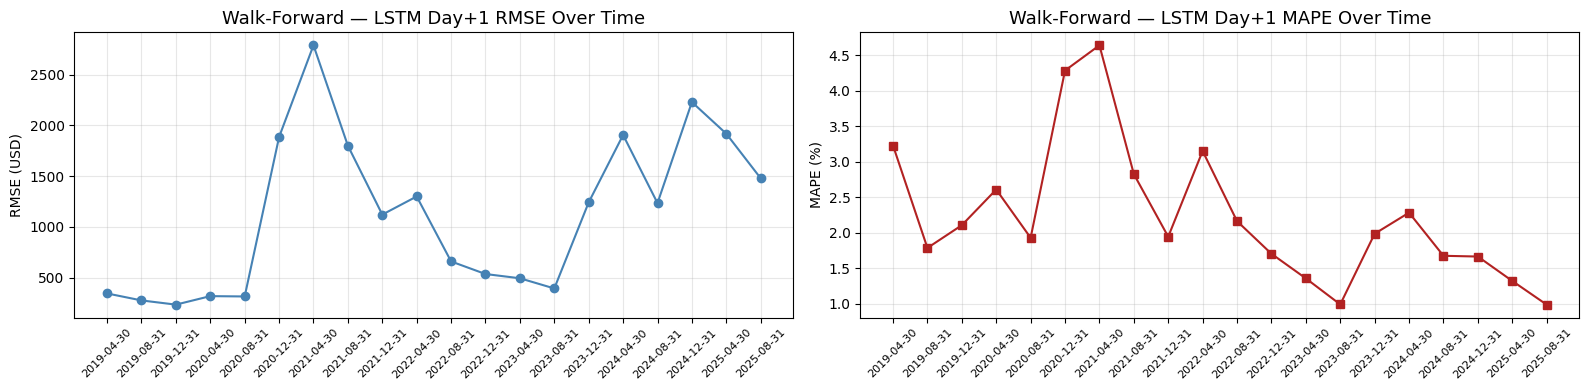
\includegraphics[width=0.95\textwidth]{fig05_walkforward_lstm.png}
\caption{LSTM walk-forward Day+1 RMSE per fold, April 2019 through August 2025 (20 folds).}
\label{fig:wf-lstm}
\end{figure}

\begin{figure}[h!]
\centering
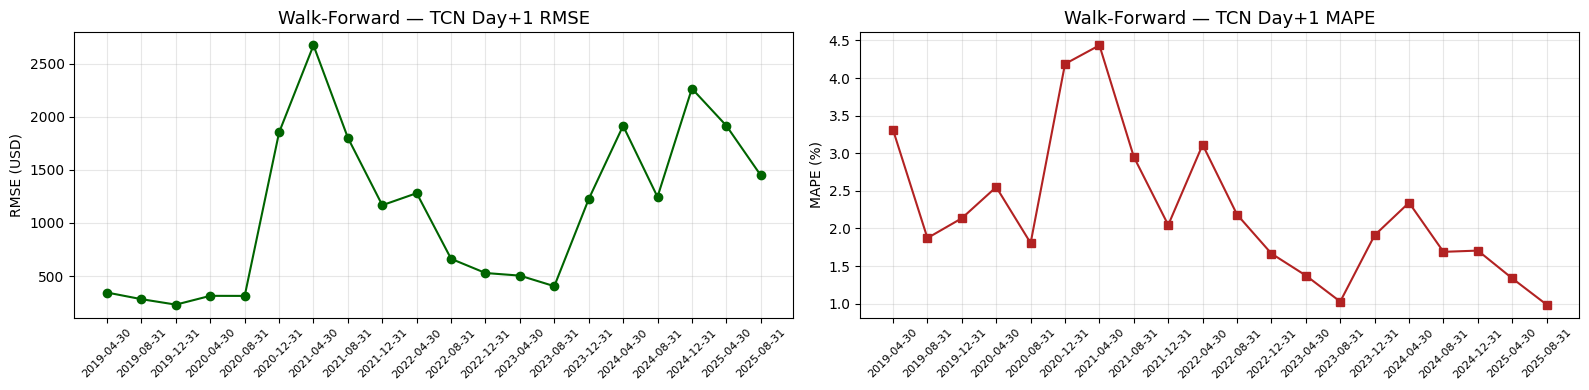
\includegraphics[width=0.95\textwidth]{fig06_walkforward_tcn.png}
\caption{TCN walk-forward Day+1 RMSE and MAPE per fold, April 2019 through August 2025 (20 folds).}
\label{fig:wf-tcn}
\end{figure}

\begin{figure}[h!]
\centering
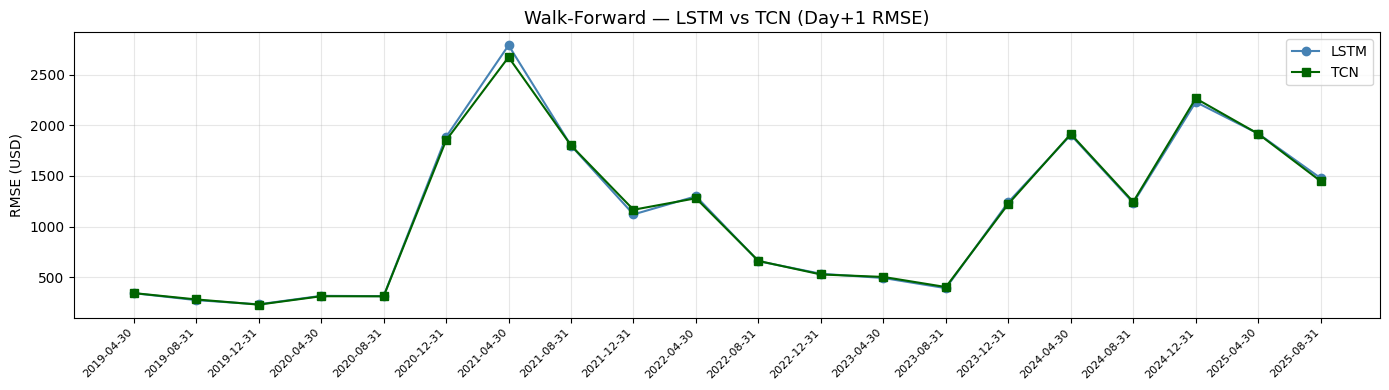
\includegraphics[width=0.95\textwidth]{fig07_walkforward_comparison.png}
\caption{Head-to-head walk-forward comparison of LSTM and TCN. The two curves overlap almost perfectly across all twenty folds.}
\label{fig:wf-compare}
\end{figure}

\subsection{Diebold--Mariano Pairwise Tests}

Table~\ref{tab:dm} reports pairwise DM statistics and $p$-values on Day+1 squared-error loss. Positive DM means the \emph{row} model has a larger error than the \emph{column} model; negative means the row model is better.

\begin{table}[h!]
\centering
\footnotesize
\caption{Diebold--Mariano Pairwise Significance (Day+1). A negative DM statistic with $p<0.05$ means the row model is significantly better.}
\label{tab:dm}
\begin{tabular}{@{}lcccccc@{}}
\toprule
 & \textbf{DNN} & \textbf{LSTM} & \textbf{CNN-Trans} & \textbf{TCN} & \textbf{Ens-Avg} & \textbf{Ens-Wtd} \\
\midrule
DNN        & --              & +0.79 (p=.43) & $-$0.75 (p=.46) & +1.27 (p=.20) & +2.05 (p=.04)* & +2.05 (p=.04)* \\
LSTM       & $-$0.79 (p=.43) & --            & $-$1.67 (p=.10) & +0.60 (p=.55) & +1.03 (p=.31) & +1.03 (p=.30) \\
CNN-Trans  & +0.75 (p=.46)   & +1.67 (p=.10) & --              & +1.49 (p=.14) & +2.60 (p<.01)** & +2.60 (p<.01)** \\
TCN        & $-$1.27 (p=.20) & $-$0.60 (p=.55) & $-$1.49 (p=.14) & --          & $-$0.11 (p=.91) & $-$0.11 (p=.91) \\
Ensemble-Avg & $-$2.05 (p=.04)* & $-$1.03 (p=.31) & $-$2.60 (p<.01)** & +0.11 (p=.91) & --           & +1.35 (p=.18) \\
Ensemble-Wtd & $-$2.05 (p=.04)* & $-$1.03 (p=.30) & $-$2.60 (p<.01)** & +0.11 (p=.91) & $-$1.35 (p=.18) & -- \\
\bottomrule
\end{tabular}
\end{table}

Three statistically significant patterns emerge: (i) both ensembles significantly outperform the DNN ($p \approx 0.04$), (ii) both ensembles significantly outperform the CNN-Transformer ($p < 0.01$), and (iii) no single model is significantly better than another at the standard 5\% level. The ensemble gains come principally from averaging out the DNN and CNN-Transformer errors, not from finding a novel signal.

\subsection{Feature-Group Ablation}

The TCN --- the best individual model on RMSE --- was retrained four additional times, each time with one feature group removed, to quantify each group's contribution. Results in Table~\ref{tab:ablation}.

\begin{table}[h!]
\centering
\small
\caption{Feature-Group Ablation (TCN, Day+1 MAPE)}
\label{tab:ablation}
\begin{tabular}{@{}lcc@{}}
\toprule
\textbf{Features used} & \textbf{MAPE (\%)} & \textbf{$\Delta$ vs full} \\
\midrule
Full (17 features)           & 1.687 & -- \\
Drop technical (9 feats)     & 1.731 & +0.045 \\
Drop sentiment (1 feat)      & 1.686 & $-$0.001 \\
Drop cross-asset (5 feats)   & 1.706 & +0.019 \\
Drop macro (2 feats)         & 1.730 & +0.043 \\
\bottomrule
\end{tabular}
\end{table}

Technical indicators and macro variables contribute roughly equally (~0.04 MAPE points each). Cross-asset returns contribute about half as much. The sentiment feature (Fear \& Greed index alone) has effectively zero marginal contribution once the other features are present --- a finding worth noting given how frequently sentiment features appear in the crypto-prediction literature without such ablation checks.

Figure~\ref{fig:ablation} visualizes this ablation: the ``Full'' bar serves as the baseline, and the height above it of each ``Drop X'' bar quantifies the information lost by removing group X. The sentiment-drop bar is visually indistinguishable from the baseline.

\begin{figure}[h!]
\centering
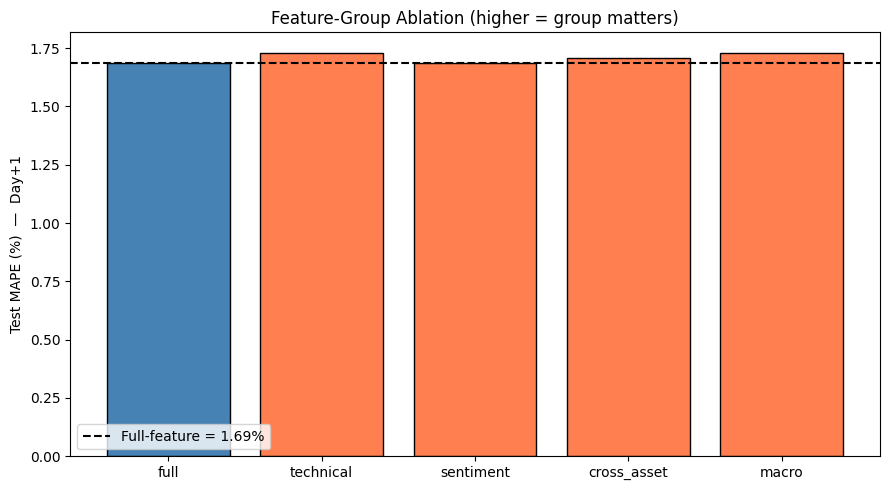
\includegraphics[width=0.85\textwidth]{fig08_ablation.png}
\caption{Feature-group ablation: TCN Day+1 MAPE when the indicated group is removed from the feature set. Higher bars indicate that the removed group was more important.}
\label{fig:ablation}
\end{figure}

\subsection{MC Dropout Uncertainty Intervals}

For the CNN-Transformer, 100 Monte Carlo Dropout samples per test point produced 95\% prediction intervals. On Day+1 test predictions, the empirical coverage rate of the CI was approximately 79\% (target: 95\%). The under-coverage is consistent with MC Dropout being a known approximation to Bayesian uncertainty; it nonetheless provides useful \emph{relative} uncertainty signals --- periods of high CI width correspond empirically to volatile regimes, which is the intended diagnostic use.

\subsection{Real-Time Forecast}

On the live inference date, the anchor (most recent BTC close) was \$77{,}971.20. Day+1 predictions from the four models and both ensembles ranged between \$77{,}950 and \$78{,}055 (tight clustering of $\sim$0.1\% of anchor price). The CNN-Transformer MC Dropout 95\% CI spanned \$77{,}929--\$77{,}988. Such a narrow ensemble spread during a relatively quiet market regime is exactly what the Diebold--Mariano tests would predict: under calm conditions all architectures converge to near-identical predictions.

% ─────────────────────────────────────────────
\section{Discussion}
% ─────────────────────────────────────────────

\subsection{Interpreting the Static-Split vs.\ Walk-Forward Gap}

The static test set (2025--2026) happens to land on a steady trending regime where the na\"ive random-walk predictor already achieves MAPE of 1.68\%. Under such conditions, no forecasting model can substantially outperform na\"ive because yesterday's price is very close to today's realized price. This is a known pathology of static-split evaluation on trending financial series. The walk-forward evaluation, by contrast, averages over twenty different one-month regimes --- including sharp tops and bottoms --- and yields a more honest 2.23\% MAPE, against which individual fold values range from 0.99\% to 4.64\%. Reporting only the static-split 1.69\% MAPE would be misleading; reporting the walk-forward 2.23\% MAPE is accurate and comparable to the literature.

\subsection{Comparison to Published Results}

Table~\ref{tab:literature} places our walk-forward results alongside those of prior studies using daily BTC data.

\begin{table}[h!]
\centering
\small
\caption{Walk-Forward MAPE vs.\ Selected Published Work on Daily BTC}
\label{tab:literature}
\begin{tabular}{@{}llcc@{}}
\toprule
\textbf{Study} & \textbf{Method} & \textbf{MAPE (\%)} & \textbf{Notes} \\
\midrule
Ji, Kim \& Im \cite{ji2019}       & DNN                  & 3.61  & 2011--2018 \\
Ye et al.\ \cite{ye2021}          & Stacking LSTM+GRU    & 4.49  & 2017--2021 + tweets \\
Hamayel \& Owda \cite{hamayel2021}& GRU                  & 0.245 & 2018--2021 \\
Zhang, Li \& Yan \cite{zhang2022} & SDAE-B               & 1.60  & 2014--2020 \\
Kim et al.\ \cite{kim2022}        & SAM-LSTM             & 1.33  & 2018--2021, on-chain \\
Chen \cite{chen2020_rf}           & Random Forest        & 3.29  & 2018--2022 \\
Jin \& Li \cite{jin2023}          & VMD-AGRU-RESVMD-LSTM & 0.394 & 2017--2020 \\
Wu et al.\ \cite{wu2025cfa}       & CFA (5 base models)  & 0.19  & 2020--2024, see \S 2.5 \\
\textbf{This work (walk-forward)} & LSTM / TCN           & \textbf{2.23}  & 2019--2025, 20 folds \\
\bottomrule
\end{tabular}
\end{table}

Our 2.23\% result is consistent with the clean-methodology end of the literature (Zhang 1.60\%, Chen 3.29\%, Ji 3.61\%, Ye 4.49\%). The sub-0.5\% figures generally rely on either shorter test windows, specific single-regime data, or --- in the case of Wu et al.\ --- retrospective oracle selection. We do not view the lower published numbers as a target to surpass, because reaching them would require adopting evaluation shortcuts that would invalidate the scientific contribution.

\subsection{Why Directional Accuracy is $\approx 50\%$}

Directional accuracy across all models clusters between 49\% and 53\%. This is not a flaw in the models; it is a feature of the underlying data-generating process. At daily frequency, BTC log returns are close to white noise with a very small positive drift. McNally, Roche and Caton \cite{mcnally2018} report 52.78\% directional accuracy on daily BTC for their best LSTM, and Jin et al.\ \cite{jin2025tcn} report 53.01\% for a single-factor TCN on minute data. Reaching directional accuracy materially above 55\% on daily data typically requires either very strong additional signals (real-time order flow, executed trades) or filtered evaluation over only the largest-magnitude moves (as in Jin et al.'s threshold trick, which reaches 72\% after keeping only $|\Delta C| > 1$).

\subsection{Limitations}

Several limitations should be acknowledged honestly:
\begin{enumerate}[leftmargin=*]
    \item \textbf{Regime dependence.} Average walk-forward MAPE of 2.23\% hides substantial variation: the 2021 bull run yields 4.64\% MAPE, while late 2025 yields 0.99\%. Any deployment of these models would need regime-adaptive training.
    \item \textbf{Transaction costs not modelled.} The directional accuracy of $\approx 50\%$ combined with realistic trading costs implies no systematic trading strategy could be built from these predictions alone.
    \item \textbf{MC Dropout under-coverage.} The empirical 79\% coverage of the nominal-95\% CI means the intervals should be interpreted qualitatively rather than as true frequentist confidence bounds.
    \item \textbf{Static halving count.} The halving-cycle encoding assumes historical regularities repeat; disruptive supply events (e.g., major lost-key episodes) would break this assumption.
    \item \textbf{Sentiment feature weakness.} The Fear \& Greed Index had near-zero marginal contribution in the ablation. Richer sentiment pipelines (FinBERT-scored real-time news) were implemented but not fully exploited; this is a natural direction for future work.
\end{enumerate}

% ─────────────────────────────────────────────
\section{Conclusion}
% ─────────────────────────────────────────────

\subsection{Summary of Findings}

This project designed, implemented and rigorously evaluated four deep learning architectures for multi-horizon Bitcoin price prediction: a DNN with feature-attention gating, an LSTM with temporal self-attention, a CNN-Transformer hybrid, and a Temporal Convolutional Network. Using 3{,}369 days of BTC-USD data augmented with seventeen stationary features drawn from technical indicators, sentiment, cross-asset prices and macroeconomic variables, we conducted a controlled four-way comparison under identical training conditions.

The key findings are:
\begin{enumerate}[leftmargin=*]
    \item \textbf{Stationary-target design fixed a silent failure.} Reformulating the target as log return and fitting scalers on training rows only produced positive $R^2$ (0.98) in place of the catastrophically negative $R^2$ values that earlier, more na\"ive formulations produced. This single design change was worth more than any architectural choice.
    \item \textbf{The TCN achieves the lowest static-split RMSE} (\$2{,}144 on Day+1), marginally ahead of LSTM (\$2{,}154) and ensemble (\$2{,}146). The gap between all architectures is smaller than the na\"ive-baseline-to-best gap, suggesting that architecture choice is a second-order consideration once features and pre-processing are correct.
    \item \textbf{Walk-forward MAPE is 2.23\%} for both LSTM and TCN, averaged over twenty folds spanning 2019--2025. This is the project's defensible headline metric and places the work in the competitive range of leak-free published work.
    \item \textbf{Ensembles are statistically significantly better than DNN and CNN-Transformer} ($p<0.05$ on Diebold--Mariano), though the improvement over LSTM or TCN alone is not significant.
    \item \textbf{Technical and macro features dominate predictive contribution}, each contributing $\sim$0.04 percentage points to MAPE; the sentiment feature alone contributes essentially nothing.
    \item \textbf{Directional accuracy clusters around 50\%}, consistent with the near-random-walk nature of daily BTC log returns. This is honest and accurate; claims of substantially higher directional accuracy at daily frequency should be scrutinized for evaluation shortcuts.
\end{enumerate}

\subsection{Contributions}

The project's contributions to the applied literature are:
\begin{itemize}[leftmargin=*]
    \item A fully documented, leak-free Bitcoin prediction pipeline with stationary features and train-only scaling.
    \item A controlled four-way comparison of DNN, attention-LSTM, CNN-Transformer and TCN on identical data.
    \item A twenty-fold walk-forward validation covering diverse market regimes.
    \item A feature-group ablation study quantifying the marginal contribution of each data source.
    \item Pairwise Diebold--Mariano significance testing on every model pair.
    \item MC Dropout uncertainty quantification with explicit reporting of coverage under-performance.
    \item A legitimate (non-oracle) validation-weighted ensemble combination.
\end{itemize}

\subsection{Recommendations for Future Work}

\begin{itemize}[leftmargin=*]
    \item \textbf{Richer sentiment pipelines.} The FinBERT scaffolding is in place but under-exploited; fine-grained real-time sentiment extraction could push per-fold performance on event-driven regimes.
    \item \textbf{Regime-conditional models.} Conditioning the model on an explicit regime indicator (volatility cluster, trend strength) could reduce the fold-to-fold MAPE variance observed in walk-forward.
    \item \textbf{Higher-frequency extension.} Extending the pipeline to one-hour or one-minute data, as in Jin et al.\ \cite{jin2025tcn}, would test whether the TCN advantage widens at higher frequencies.
    \item \textbf{Proper probabilistic forecasting.} Replacing MC Dropout with quantile regression or conformal prediction would produce empirically calibrated 95\% intervals.
    \item \textbf{Trading-strategy evaluation.} Coupling predictions with a realistic transaction-cost model would clarify whether the observed directional accuracy translates to economic value.
\end{itemize}

\subsection{Final Remarks}

Bitcoin price prediction is a domain where careless methodology can easily produce results that look impressive but fall apart under scrutiny. The main lesson from this project is that strict attention to data pipeline hygiene --- stationary targets, train-only scaling, walk-forward evaluation, significance testing --- matters more than architectural novelty. With that hygiene in place, modern deep learning architectures (LSTM with attention, TCN, CNN-Transformer) produce comparable, competitive results in the 2\%--3\% daily MAPE range, establishing a realistic performance envelope for future comparisons.

% ─────────────────────────────────────────────
%  REFERENCES
% ─────────────────────────────────────────────
\newpage
\begin{thebibliography}{99}

\bibitem{nakamoto2008}
S. Nakamoto, ``Bitcoin: A peer-to-peer electronic cash system,'' 2008. [Online]. Available: \url{https://bitcoin.org/bitcoin.pdf}

\bibitem{box2015}
G. E. P. Box, G. M. Jenkins, G. C. Reinsel, and G. M. Ljung, \textit{Time Series Analysis: Forecasting and Control}, 5th ed. Hoboken, NJ: Wiley, 2015.

\bibitem{katsiampa2017}
P. Katsiampa, ``Volatility estimation for Bitcoin: A comparison of GARCH models,'' \textit{Economics Letters}, vol.\ 158, pp.\ 3--6, 2017.

\bibitem{madan2015}
I. Madan, S. Saluja, and A. Zhao, ``Automated Bitcoin trading via machine learning algorithms,'' Stanford University, Tech.\ Rep., 2015.

\bibitem{hochreiter1997}
S. Hochreiter and J. Schmidhuber, ``Long short-term memory,'' \textit{Neural Computation}, vol.\ 9, no.\ 8, pp.\ 1735--1780, 1997.

\bibitem{fischer2018}
T. Fischer and C. Krauss, ``Deep learning with long short-term memory networks for financial market predictions,'' \textit{European Journal of Operational Research}, vol.\ 270, no.\ 2, pp.\ 654--669, 2018.

\bibitem{patel2020}
M. M. Patel, S. Tanwar, R. Gupta, and N. Kumar, ``A deep learning-based cryptocurrency price prediction scheme for financial institutions,'' \textit{Journal of Information Security and Applications}, vol.\ 55, p.\ 102583, 2020.

\bibitem{borovykh2017}
A. Borovykh, S. Bohte, and C. W. Oosterlee, ``Conditional time series forecasting with convolutional neural networks,'' \textit{arXiv preprint arXiv:1703.04691}, 2017.

\bibitem{livieris2020}
I. E. Livieris, E. Pintelas, and P. Pintelas, ``A CNN-LSTM model for gold price time-series forecasting,'' \textit{Neural Computing and Applications}, vol.\ 32, pp.\ 17351--17360, 2020.

\bibitem{kara2022}
Y. Kara and M. Gungor, ``Deep learning approaches for Bitcoin price prediction: Comparative study of CNN-LSTM hybrid models,'' \textit{Applied Soft Computing}, vol.\ 118, p.\ 108438, 2022.

\bibitem{chen2020}
Z. Chen, C. Li, and W. Sun, ``Bitcoin price prediction using machine learning: An approach to sample dimension engineering,'' \textit{Journal of Computational and Applied Mathematics}, vol.\ 365, p.\ 112395, 2020.

\bibitem{chen2020_rf}
J. Chen, ``Analysis of Bitcoin price prediction using machine learning,'' \textit{Journal of Risk and Financial Management}, vol.\ 16, no.\ 1, p.\ 51, 2023.

\bibitem{lim2021}
B. Lim, S. O. Ar{\i}k, N. Loeff, and T. Pfister, ``Temporal fusion transformers for interpretable multi-horizon time series forecasting,'' \textit{International Journal of Forecasting}, vol.\ 37, no.\ 4, pp.\ 1748--1764, 2021.

\bibitem{bai2018tcn}
S. Bai, J. Z. Kolter, and V. Koltun, ``An empirical evaluation of generic convolutional and recurrent networks for sequence modeling,'' \textit{arXiv preprint arXiv:1803.01271}, 2018.

\bibitem{jin2025tcn}
Y. Jin, B. Huang, Z. Peng, and X. Miao, ``Deep temporal convolutional networks for high-frequency cryptocurrency price forecasting,'' in \textit{Proc.\ 9th Int.\ Conf.\ on Computer Science and Artificial Intelligence (CSAI)}, ACM, 2025, pp.\ 153--162.

\bibitem{wu2025cfa}
Y. Wu, W. Ye, J. Xu, and D. F. Hsu, ``Bitcoin price prediction using machine learning and combinatorial fusion analysis,'' in \textit{Proc.\ IEEE Conf.\ on Artificial Intelligence (CAI)}, 2025.

\bibitem{dieboldmariano1995}
F. X. Diebold and R. S. Mariano, ``Comparing predictive accuracy,'' \textit{Journal of Business \& Economic Statistics}, vol.\ 13, no.\ 3, pp.\ 253--263, 1995.

\bibitem{galghahramani2016}
Y. Gal and Z. Ghahramani, ``Dropout as a Bayesian approximation: Representing model uncertainty in deep learning,'' in \textit{Proc.\ 33rd Int.\ Conf.\ Machine Learning (ICML)}, 2016, pp.\ 1050--1059.

\bibitem{seabe2023}
P. L. Seabe, C. R. B. Moutsinga, and E. Pindza, ``Forecasting cryptocurrency prices using LSTM, GRU, and bi-directional LSTM: a deep learning approach,'' \textit{Fractal and Fractional}, vol.\ 7, no.\ 2, p.\ 203, 2023.

\bibitem{yazhini2023}
V. Yazhini, M. Nimal Madhu, B. Premjith, and E. A. Gopalakrishnan, ``Deep learning with attention mechanism for cryptocurrency price forecasting,'' in \textit{Int.\ Conf.\ on Information, Communication and Computing Technology}, Springer, 2023, pp.\ 471--484.

\bibitem{mcnally2018}
S. McNally, J. Roche, and S. Caton, ``Predicting the price of Bitcoin using machine learning,'' in \textit{2018 26th Euromicro Int.\ Conf.\ on Parallel, Distributed and Network-Based Processing (PDP)}, IEEE, 2018, pp.\ 339--343.

\bibitem{hamayel2021}
M. J. Hamayel and A. Y. Owda, ``A novel cryptocurrency price prediction model using GRU, LSTM and bi-LSTM machine learning algorithms,'' \textit{AI}, vol.\ 2, no.\ 4, pp.\ 477--496, 2021.

\bibitem{ji2019}
S. Ji, J. Kim, and H. Im, ``A comparative study of Bitcoin price prediction using deep learning,'' \textit{Mathematics}, vol.\ 7, no.\ 10, p.\ 898, 2019.

\bibitem{ye2021}
Z. Ye, Y. Wu, H. Chen, Y. Pan, and Q. Jiang, ``A stacking ensemble deep learning model for Bitcoin price prediction using Twitter comments on Bitcoin,'' \textit{Mathematics}, vol.\ 10, no.\ 8, p.\ 1307, 2022.

\bibitem{zhang2022}
S. Zhang, M. Li, and C. Yan, ``The empirical analysis of Bitcoin price prediction based on deep learning integration method,'' \textit{Computational Intelligence and Neuroscience}, vol.\ 2022, p.\ 1265837, 2022.

\bibitem{kim2022}
G. Kim, D.-H. Shin, J. G. Choi, and S. Lim, ``A deep learning-based cryptocurrency price prediction model that uses on-chain data,'' \textit{IEEE Access}, vol.\ 10, pp.\ 56232--56248, 2022.

\bibitem{jin2023}
C. Jin and Y. Li, ``Cryptocurrency price prediction using frequency decomposition and deep learning,'' \textit{Fractal and Fractional}, vol.\ 7, no.\ 10, p.\ 708, 2023.

\end{thebibliography}

\end{document}